\section{Experimental Setup}
\label{sec:exp_setup}
\subsection{Distillation Process} We observe that the output scores from the dual-encoder and the cross-encoder models are not bounded to specific intervals. Hence, we do min-max normalization separately on the query vector's scores $Q^T_q\hat{P}$ (from the dual-encoder) and the cross encoder's scores $R(q,P)$ to bring the two scoring distributions closer. Further, the cross-encoder tends to have peaky scoring distributions, hence we use a temperature $T$ (= 2 after tuning) while computing the softmax $D_{CE}(q,P)$ over the cross-encoder scores. After tuning on the MS Marco dev set, we set the number of updates $n$=100 with learning rate $\alpha$=0.005.

\subsection{Rerank Baseline}
\begin{table}
%\vspace{-1em}  
\small
\setlength{\tabcolsep}{1.0em}
        \centering
        \def\arraystretch{1.3}
        \begin{tabular}{c|cc|c}
        \hline
        \multirow{2}{*}{\textbf{Step (Device)}} & \multicolumn{2}{c}{\textbf{Retrieve \& Rerank}} & \multirow{2}{*}{\parbox{3em}{\centering\textbf{\textsc{ReFIT} (K=100)}}}\\
        \cline{2-3}
        & \multicolumn{1}{|c}{\textbf{K=100}} & \multicolumn{1}{c|}{\textbf{K=125}} & \\
        \hline
        1st Retrieval (CPU) & \multicolumn{1}{c}{40ms} & \multicolumn{1}{c|}{40ms} & \multicolumn{1}{c}{40ms} \\
        \hdashline
        Rerank (CPU) & \multicolumn{1}{c}{1540ms} & \multicolumn{1}{c|}{1925ms} & \multicolumn{1}{c}{1540ms} \\
        Rerank (GPU) & \multicolumn{1}{c}{360ms} & \multicolumn{1}{c|}{450ms} & \multicolumn{1}{c}{360ms} \\
        %\hline
        \hdashline
        Distillation (CPU) & \multicolumn{1}{c}{-} & \multicolumn{1}{c|}{-}&  \multicolumn{1}{c}{30ms}\\
        %\hline
        2nd Retrieval (CPU) & \multicolumn{1}{c}{-} & \multicolumn{1}{c|}{-} & \multicolumn{1}{c}{40ms}\\
        \hline
        Total (CPU) & \multicolumn{1}{c}{1580ms}&  \multicolumn{1}{c|}{1965ms} & \multicolumn{1}{c}{1650ms}\\
        Total (GPU) & \multicolumn{1}{c}{400ms}&  \multicolumn{1}{c|}{490ms} & \multicolumn{1}{c}{470ms}\\
        \hline
        \end{tabular}
        \caption{Comparison of inference times (in milliseconds) for different approaches, utilizing both CPU-only and GPU configurations (when reranking $K$ passages).}
        \label{tab:inf_times}
        \vspace{-1em}    
\end{table}

\textsc{ReFIT} introduces the additional overhead of distillation and a second retrieval step into the R\&R framework. We note that distillation latency (in Algorithm \ref{alg4}) in linear in the number of updates $n$.
Table \ref{tab:inf_times} compares the inference latency of our method with that of standard R\&R, assuming $K$=100 passages are to be reranked and $n$=100 updates are used during distillation. We highlight that our distillation process is lightweight and takes just 30ms on a CPU. We see that the additional distillation and retrieval steps increase the latency of inference by roughly 17.5\% when using a GPU (or 4.4\% for CPU);\footnote{24-core AMD EPYC 7352 CPU and 80GB A100 GPU.} in that same amount of time, vanilla R\&R can process a total of 125 passages on the GPU (see Table~\ref{tab:inf_times}), to potentially increase Recall@100. Hence, and for fair comparison, we evaluate against a \mbox{\textit{Rerank}} baseline that is allowed to retrieve and rerank 125 passages. 
We note that both \textsc{ReFIT} and the \textit{Rerank} baseline use the same retriever and reranker, and are evaluated on Recall@100. 

\subsection{Retriever and Reranker} 
\label{sec:retriever_and_reranker}
We use Contriever \cite{izacard2021unsupervised} as the underlying retriever (unless otherwise mentioned), which has been pre-trained with an unsupervised contrastive learning objective on a large-scale collection of Wikipedia and CCNet documents. Contriever is a dual-encoder retriever that outperforms  traditional term-matching methods, BM25 and recent dense approaches e.g. DPR \cite{karpukhin2020dense} and ANCE \cite{xiong2020approximate}.
For retrieval in both English and other languages, we use the publicly available version of Contriever, fine-tuned on MS MARCO \cite{nguyen2016ms}. Our English\footnote{\href{https://huggingface.co/cross-encoder/ms-marco-MiniLM-L-6-v2}{cross-encoder/ms-marco-MiniLM-L-6-v2}} and multilingual\footnote{\href{https://huggingface.co/cross-encoder/mmarco-mMiniLMv2-L12-H384-v1}{cross-encoder/mmarco-mMiniLMv2-L12-H384-v1}} rerankers are based on sentence transformers. 

\section{Results}
\label{sec:results}

\subsection{English Retrieval in Multiple Domains}
\label{sec:english_results}


\begin{table*}[t]
    \centering
    \scriptsize
    \setlength{\tabcolsep}{0.3em}
    \def\arraystretch{1.3}
    \begin{tabular}{c|cc:cccc|ccc}
    \hline
    \multicolumn{1}{c|}{\multirow{2}{*}{}} & \multicolumn{1}{c}{\multirow{2}{*}{\textbf{BM25}}} & \multicolumn{1}{c:}{\multirow{2}{*}{\textbf{ANCE}}} & \multicolumn{1}{c}{\multirow{2}{*}{\textbf{RocketQA}}} & \multicolumn{1}{c}{\multirow{2}{*}{\textbf{RocketQA}}} & \multicolumn{1}{c}{\textbf{RocketQA}}& \multicolumn{1}{c|}{\textbf{RocketQA}} & \multicolumn{1}{c}{\multirow{2}{*}{\textbf{Contriever}}} & \multicolumn{1}{c}{\textbf{Contriever}}& \multicolumn{1}{c}{\textbf{Contriever}}  \\
  & & & \textbf{v1} & \textbf{v2} & \textbf{v1+Rerank} &  \textbf{v1+\textsc{ReFIT}} & &  \textbf{+ Rerank} &  \textbf{+ \textsc{ReFIT}}  \\
    \hline
     MS MARCO & 65.8 &  85.2 & 88.4 & 88.7&	89.4& \textbf{90.0*}   & 89.1 & 89.9  & \textbf{90.5}* \\
       Trec-COVID  & 49.8  & 45.7  &48.5&	46.4&	52.0&	\textbf{52.9}   &  40.7 & 43.8  & \textbf{51.5}*\\
       NFCorpus   & 25.0   & 23.2 & 26.9	&25.9&	27.4	&\textbf{29.2*} & 30.0  & 29.5 & \textbf{31.9}*\\
       NQ  & 76.0 & 83.6 & 91.1	&89.8	&91.8	&\textbf{92.7*}  &  92.5 &  93.3  & \textbf{94.2}*\\
       HotpotQA  & 74.0 &  57.8   & 69.8	&67.7	&71.4	&\textbf{73.3*}   & 77.7 & 78.6  & \textbf{80.4}*\\
       FiQA  & 53.9   & 58.1 & 63.6	&61.2	&\textbf{64.3}	&63.8   & 65.6 &  \textbf{65.9}  & 65.6 \\
       DBPedia  & 39.8  &  31.9 & 45.7	&43.4	&47.6	&\textbf{50.2*}  &  54.1 & 56.0  & \textbf{57.3}*\\
       Scidocs & 35.6  &  26.9 & 31.8	&29.3	&33.1	&\textbf{35.5*}  &  37.8  & 38.3 & \textbf{40.1}*\\
       FEVER &  93.1   & 90.0 & 92.6	&92.5	&92.8	&\textbf{93.7*}   & 94.9 &  95.3  & \textbf{95.5}*\\
       Climate-FEVER  & 43.6   & 44.5  & 47.4	&48.7	&49.3&	\textbf{53.6*}    & 57.4  & 59.0  & \textbf{59.5}\\
       Scifact   & 90.8  & 81.6  & 88.1	&85.4	&89.0	&\textbf{89.9*}  & 94.7&  94.4 & \textbf{95.2*}\\
       \hline
       Average& 58.9  & 57.1 & 63.1	&61.7	&64.4	&\textbf{65.9*}  & 66.8 & 67.6  & \textbf{69.0}* \\
       \hline
    \end{tabular}
    %\vspace{1em}
    \caption{Recall@100 (in \%) on the English BEIR benchmark. Performance of \textsc{ReFIT} is shown for different choices of underlying retrievers. RocketQAv2~\cite{ren2021rocketqav2} corresponds to a training-time distillation baseline. Improvements marked with * are statistically significant at $p<0.05$ as per paired t-test.}
    \label{tab:beir_nums}
\end{table*}

We evaluate English retrieval performance on the BEIR benchmark \cite{thakur2021beir}, comprising training and in-domain test instances from MS MARCO and out-of-domain evaluation data from a number of scientific, biomedical, financial, and Wikipedia-based retrieval datasets\footnote{We omit some datasets due to license \& versioning issues.}. 

Firstly, we compare our inference-time distillation approach against a training-time distillation method. We use RocketQAv1~\cite{qu-etal-2021-rocketqa} as the underlying retrieval model and RocketQAv2~\cite{ren-etal-2021-rocketqav2} as the retriever distilled at training time from the cross-encoder. We also compare with a \textit{Rerank} (K=125) baseline, which improves Recall@100 by reranking the top 125 passages (retrieved by RocketQAv1). Moreover, we also demonstrate the effectiveness of \textsc{ReFIT} with a different underlying retrieval model, in this case, Contriever.

\begin{table}[t]
\scriptsize
    \centering
    \setlength{\tabcolsep}{1.0em}
    \def\arraystretch{1.3}
    \begin{tabular}{c|cc:ccc}
    \hline
    & \multicolumn{1}{c}{\parbox{2.8em}{\textbf{mBERT}}}  & \multicolumn{1}{c:}{\parbox{4em}{\textbf{XLM-R}}} & \multicolumn{1}{c}{\parbox{4em}{\textbf{Contriever}}} & \multicolumn{1}{c}{\parbox{3em}{\textbf{Rerank}}} & \multicolumn{1}{c}{\parbox{3em}{\textbf{\textsc{ReFIT}}}} \\
    \hline
    Arabic  & 81.1  & 79.9   & 88.7 &   89.5  &\textbf{90.9}* \\
    Bengali  &88.7   & 84.2   & 91.4&    91.4   & \textbf{95.9}* \\
    English  & 77.8    &  73.1  & 77.2&   78.7  &  \textbf{81.8}* \\
    Finnish   & 74.2   &  81.6  & 88.1 &    88.9  &\textbf{91.0}*\\
    Indonesian  & 81.0 & 87.4  & 89.8 &  90.5 &\textbf{93.7}*\\
    Japanese  & 76.1  &  70.9  & 81.7 & 82.5  &\textbf{85.2}*\\
    Korean  & 66.7  & 71.1  & 78.2&    \textbf{81.0}  &80.2\\
    Russian& 77.6  & 74.1    & 83.8 &   85.7  & \textbf{87.3}\\
    Swahili & 74.1 & 73.9   & 91.4  &  \textbf{92.0} &90.5\\
    Telugu & 89.5 & 91.2  & 96.6&    97.0 & \textbf{97.5}\\
    Thai& 57.8  &  89.5   & 90.5&    91.6  &\textbf{93.3}*\\
    \hline
    Average  & 76.8  & 79.7 & 87.0&   88.1 & \textbf{89.7}*\\
    \hline
    \end{tabular}
    %\vspace{1em}
    \caption{Recall@100 (in \%) on the multilingual Mr.TyDi benchmark. Rerank and \textsc{ReFIT} use Contriever as the underlying retriever. * corresponds to statistical significance at $p<0.05$ (paired t-test).}
    \label{tab:mrtydi_nums}
    \vspace{-1em}
\end{table}

Table \ref{tab:beir_nums} shows Recall@100 results on the BEIR benchmark. Firstly, we see that \textsc{ReFIT} consistently outperforms all baselines. Next, RocketQAv2 shows improvement over RocketQAv1 on MS MARCO, which is the dataset used for training-time distillation of RocketQAv2. However, RocketQAv2's performance degrades on out-of-domain datasets from the BEIR benchmark. This is unsurprising, since the training-time distillation approach is limited to the bi-encoder seeing the cross-encoder’s relevance labels only in the source domain, i.e. the domain used for training (MS MARCO in this case). As a result, the training-time distillation approach may not generalize well to unseen domains (BEIR in this case). In contrast, \textsc{ReFIT} offers the key advantage of learning from target-domain pseudo labels provided by the reranker \textit{at inference}, which yields improved out-of-domain generalization.

\subsection{Retrieval in More Languages}
\label{sec:multilingual_results}

\subsubsection{Multilingual Retrieval}
 We also evaluate on Mr. TyDi \cite{zhang2021mr}, a multilingual IR benchmark derived from TyDi QA \cite{clark2020tydi}, where given a question in one of 11 languages, the goal is to retrieve candidates from a pool of Wikipedia documents in the same language. Our underlying retriever is the multilingual version of Contriever. Other baseline retrieval models are mBERT and XLM-R \cite{conneau2020unsupervised}, in addition to the \textit{Rerank} (K=125) baseline. Table \ref{tab:mrtydi_nums} shows Recall@100 for the different systems on Mr.TyDi. Here again, \textsc{ReFIT} yields significant improvement over all baselines on most languages.

\subsubsection{Cross-lingual Retrieval}
For our cross-lingual experiments, we used the MKQA benchmark \cite{longpre2021mkqa}. MKQA involves retrieving passages from the English Wikipedia corpus for questions that are posed in 26 different languages. Following \cite{izacard2021unsupervised}, we discard unanswerable questions and questions with a yes/no answer or a long answer, leaving 6,619 queries per language in the final test set. 
Table \ref{tab:crossling_nums} compares Recall@100 of different models on MKQA. \textsc{ReFIT} again outperforms, leading the nearest baseline (\textit{Rerank}) by about 2 points on average, and with improvements on all 26 MKQA languages.

\begin{table*}[t]
    \centering
    \scriptsize
    \setlength{\tabcolsep}{0.7em}
    \def\arraystretch{1.3}
    \begin{tabular}{lcccccccccccccc}
    \hline
    & \textbf{avg} & \textbf{en} & \textbf{ar} & \textbf{fi} & \textbf{ja} & \textbf{ko} & \textbf{ru} & \textbf{es} & \textbf{sv} & \textbf{he} & \textbf{th} & \textbf{da} & \textbf{de} & \textbf{fr}\\ 
    \hline
    mBERT & 57.9 &74.2 & 44.0 & 51.7 & 55.7 &48.2 &57.4 &63.9 & 62.7 & 46.8 & 51.7 & 63.7 & 59.6 & 65.2\\
    XLM-R & 59.2 & 73.4 & 42.4 & 57.7& 53.1 &48.6 &58.5 &62.9 &67.5 &46.9 &61.5 &66.9 &60.9 &62.4\\
    \hdashline
    Contriever& 65.6 & 75.6 & 53.3 & 66.6 &60.4 &55.4 &64.7 &70.0 &70.8 &59.6 &63.5 &72.0 &66.6 &70.1\\
    Rerank & 66.4 & 76.0 & 54.5 & 67.5 & 61.5 & 56.7 & 65.8 & 70.5 & 71.6 & 60.8 & 64.9 & 72.7 & 67.5 & 70.6\\
    \textsc{ReFIT} & \textbf{68.2} & \textbf{76.6} & \textbf{58.0} & \textbf{68.8} & \textbf{64.7} & \textbf{59.3} & \textbf{68.4} & \textbf{72.5} & \textbf{73.1} & \textbf{62.9} & \textbf{66.5} & \textbf{74.1} & \textbf{70.1} & \textbf{72.5}\\
    \hline
    \hline
    &  & \textbf{it} & \textbf{nl} & \textbf{pl} & \textbf{pt} & \textbf{hu} & \textbf{vi} & \textbf{ms} & \textbf{km} & \textbf{no} & \textbf{tr} & \textbf{zh-cn} & \textbf{zh-hk} & \textbf{zh-tw} \\ 
    \hline
   mBERT & & 64.1 & 66.7 & 59.0 & 61.9 & 57.5 & 58.6 & 62.8 & 32.9 & 63.2 & 56.0 & 58.4 & 59.3 & 59.3\\
    XLM-R & & 58.1 & 66.4 & 61.0 & 62.0 & 60.1 & 62.4 & 66.1 & \textbf{46.6} & 65.9 & 60.6 & 55.8 & 55.5 & 55.7\\
    \hdashline
    Contriever & & 70.3 &71.4 &68.8 &68.5 &66.7 &67.8 &71.6 &37.8 &71.5 &68.7 &64.1 &64.5 &64.3 \\
    Rerank & & 70.8 & 72.0 & 69.9 & 69.3 & 67.5 & 68.7 & 72.0 & 38.6 & 72.3 & 69.3 & 65.1 & 65.4 & 65.2 \\
    \textsc{ReFIT} & & \textbf{72.4} & \textbf{73.6} & \textbf{71.1} & \textbf{71.5} & \textbf{68.9} & \textbf{70.5} & \textbf{73.3} & 39.9 &\textbf{73.3} & \textbf{70.7} & \textbf{67.5} & \textbf{67.4} & \textbf{66.9} \\
    \hline
    \hline
    \end{tabular}
    %\vspace{1em}
    \caption{Recall@100 (in \%) on the cross-lingual MKQA benchmark.  Rerank and \textsc{ReFIT} use Contriever as the underlying retriever. All improvements are statistically significant at $p < 0.05$ (paired t-test).}
    \label{tab:crossling_nums}
    \vspace{-0.5em}
\end{table*}


\subsection{Multi-modal Retrieval}
\label{sec:multimodal_results}
A key advantage of \textsc{ReFIT} is that it can operate independently of the choice of architecture for the bi-encoder and the cross-encoder, and is therefore not limited to working on only text input.
To demonstrate this, we apply our method to retrieval in a multi-modal setting. Specifically, we consider text-to-video retrieval, which involves retrieving videos that are relevant to a given textual query. 

The retriever and reranker for this experiment are based on BLIP \cite{li2022blip}, a state-of-the-art vision-language model that comprises two unimodal encoders and an image-grounded text encoder. 
The unimodal encoders encode image and text separately, akin to dual-encoders in text-to-text retrieval, and are trained with an Image-Text Contrastive (ITC) loss. The image-grounded text encoder injects visual information into the text encoder by incorporating a cross-attention layer, similar to a text-to-text cross-encoder, and is trained with an Image-Text Matching (ITM) loss. We refer the reader to \cite{li2022blip} for a more detailed description of BLIP's architecture and the pre-training objectives. BLIP can thus be used for retrieval with the unimodal encoders (which we refer to as BLIP$_{ITC}$), and for reranking with the image-grounded text encoder (which we refer to as BLIP$_{ITM}$). We use the output from BLIP$_{ITM}$ as the reranker distribution, which is then used to compute the distillation loss for updating the query representation that is output by BLIP$_{ITC}$. 

We evaluate using Recall@100 on the MSRVTT \cite{xu2016msr} text-to-video retrieval dataset, with BLIP$_{ITC}$ \cite{li2022blip} being our primary retrieval-only baseline along with other baselines taken from \cite{li2022blip}.
The \textit{Rerank} baseline uses BLIP$_{ITM}$ to rerank $K$=125 videos retrieved by BLIP$_{ITC}$.
Table \ref{tab:multimodal} compares performance on the 1k test split of MSRVTT. We see that BLIP$_{ITM}$ yields better ranking (as evident from higher Recall@10) than BLIP$_{ITC}$ as expected, but shows only minor gains in Recall@100. Crucially, \textsc{ReFIT} improves Recall@100 over the already strong BLIP$_{ITC}$ retriever, without a noticeable drop in Recall@10 compared to the BLIP$_{ITM}$ reranker.

\begin{minipage}[H]{.39\linewidth}
        \centering
        \scriptsize
        \setlength{\tabcolsep}{1.0em}
        \def\arraystretch{1.3}
        \begin{tabular}{l|c|c}
        \hline
            \textbf{Method} & \textbf{R@10} & \textbf{R@100} \\
            \hline
            MIL-NCE & 32.4 & - \\
            VideoCLIP  & 30.0 & - \\
            FiT  & 51.6 & - \\
            \hdashline
            BLIP$_{ITC}$ & 69.0 & 92.1 \\
            Rerank (BLIP$_{ITM}$) & 74.6 & 92.3\\
            \textsc{ReFIT} & \textbf{74.7} & \textbf{92.9} \\
            \hline
        \end{tabular}
        \captionof{table}{Recall of text-to-video retrieval methods on the MSRVTT benchmark.}
        \label{tab:multimodal}
        \vspace{1.0em}
\end{minipage}
\hfill
\begin{minipage}[H]{.50\linewidth}
        \centering
        \scriptsize
        \setlength{\tabcolsep}{1.0em}
        \def\arraystretch{1.3}
        \begin{tabular}{c|c|c|c|c}
        \hline
            & \textbf{NQ} & \textbf{EntityQ} & \textbf{BEIR}& \textbf{Mr.TyDi} \\
            \hline
            Retrieve & 86.1 & 70.1 & 66.8 & 87.0  \\
            Rerank & 86.8 & 71.2 & 67.6 & 88.1  \\
            \textsc{TouR}$_{\text{hard}}$ & 87.0$^+$ & 71.9$^+$  & 68.4 & 88.7 \\
            \textsc{TouR}$_{\text{soft}}$ & 87.2$^+$ & 72.5$^+$ & 68.1 & 88.1\\
            \hline
            \textsc{ReFIT} & \textbf{87.6} & \textbf{72.6} & \textbf{69.2} &  \textbf{89.7} \\
            \hline
        \end{tabular}
        \captionof{table}{Recall@100 numbers for comparison of \textsc{ReFIT} with both variants of \textsc{TouR}. $^+$ corresponds to numbers directly taken from~\cite{sung2023optimizing}.}
        \label{tab:tour_comparison}
        \vspace{1em}
\end{minipage}

\subsection{Comparison with \textsc{TouR}}
\label{sec:tour_comparison}

In this section, we compare the performance of \textsc{ReFIT} with \textsc{TouR} on the passage retrieval benchmarks used in \cite{sung2023optimizing}, NQ~\cite{kwiatkowski2019natural} and EntityQuestions~\cite{sciavolino-etal-2021-simple} as well as the multidomain BEIR and multilingual Mr.TyDi benchmarks. For NQ  and EntityQuestions, we use the same retriever~\cite{karpukhin2020dense} and reranker~\cite{fajcik-etal-2021-r2-d2} as in \cite{sung2023optimizing}. The retriever and the reranker for BEIR and Mr.TyDi are the same as described in \S{\ref{sec:retriever_and_reranker}}. 
In Table \ref{tab:tour_comparison}, we can see that \textsc{ReFIT} consistently outperforms both \textsc{TouR} variants across various datasets. 
We believe that the lower performance of \textsc{TouR} can be attributed to its early stopping criterion for distillation updates. Specifically, \textsc{TouR} performs relevance feedback for 3 iterations, wherein in each iteration, distillation into the query vector continues until the top-1 retrieval result has the highest reranker score (for \textsc{TouR}$_{\text{soft}}$) or is a pseudo-positive (for \textsc{TouR}$_{\text{hard}}$). 
In contrast, \textsc{ReFIT} makes more distillation updates but for only one iteration (we do $n=100$ updates, which has been tuned). 
This makes it also considerably faster than \textsc{TouR}, as each additional iteration of relevance feedback in \textsc{TouR} comes with a high computational overhead (\S{\ref{sec:related-work}}). 
We show in \S{\ref{sec:multi_iterations}} that \textsc{ReFIT} can further benefit from multiple rounds of relevance feedback with continuous improvements over the course of three iterations.

\subsection{\textsc{ReFIT} for multi-vector dense retrieval}

\begin{wraptable}{r}{0.38\linewidth}
    \centering
    \scriptsize
    \setlength{\tabcolsep}{0.5em}
    \def\arraystretch{1.3}
    \vspace{-1em}
    \begin{tabular}{c|ccc}
    \hline
     & \multicolumn{1}{c}{\textbf{ColBERTv2}}& \multicolumn{1}{c}{\textbf{Rerank}} & \multicolumn{1}{c}{\textbf{\textsc{ReFIT}}}   \\
    \hline
       NFCorpus   &  27.7 & 28.0 & \textbf{28.8}\\
       FiQA  & 62.8 &  63.7 &  \textbf{64.3}\\
       Scidocs & 35.8 & 36.6&  \textbf{38.5}\\
       Scifact   &  89.4 & \textbf{90.2} & 90.1\\
    \hline
    \end{tabular}
    \vspace{-0.6em}
    \caption{Recall@100 (in \%) on a subset of the English BEIR benchmark, with Rerank and \textsc{ReFIT} using ColBERTv2 as the underlying retriever.}  
    \label{tab:multi_vector}
    \vspace{-1em}
\end{wraptable}


Our experiments thus far have been focused on single-vector dense retrieval, where queries and passages are encoded as individual vectors.
Multi-vector retrieval models like ColBERT~\cite{khattab2020colbert, santhanam-etal-2022-colbertv2}, on the other hand, compute token-level query and passage representations, subsequently employing a late-interaction mechanism for scoring. This section explores the application of \textsc{ReFIT} to multi-vector retrieval, specifically, ColBERTv2~\cite{santhanam-etal-2022-colbertv2}.
In this case, distillation (Step 3 in Figure \ref{fig:overall_framework}) updates embeddings of individual tokens in the query. We present results in Table \ref{tab:multi_vector} on a subset\footnote{Owing to the substantially larger index size inherent to multi-vector dense retrieval, we restrict this study to subsets of BEIR with $<100k$ passages in the retrieval corpus.} of the BEIR dataset, which clearly show that \textsc{ReFIT} can be effectively extended to multi-vector dense retrieval, as it consistently surpasses the performance of the ColBERTv2 retriever and outperforms the Rerank baseline (with $K=125$) in most cases. Notably, the training of ColBERTv2~\cite{santhanam-etal-2022-colbertv2} involved the use of a reranker's scores for supervision; our results in this section thus reinforce the finding of \S{\ref{sec:english_results}} that \textsc{ReFIT}'s inference-time distillation can be superior to ordinary knowledge distillation during training.

\section{Discussion and Analysis}

This section describes additional experiments, providing further insights into \textsc{ReFIT}.

\begin{figure}[t]
    \centering
    \begin{subfigure}[c]{0.24\linewidth}
        \centering
     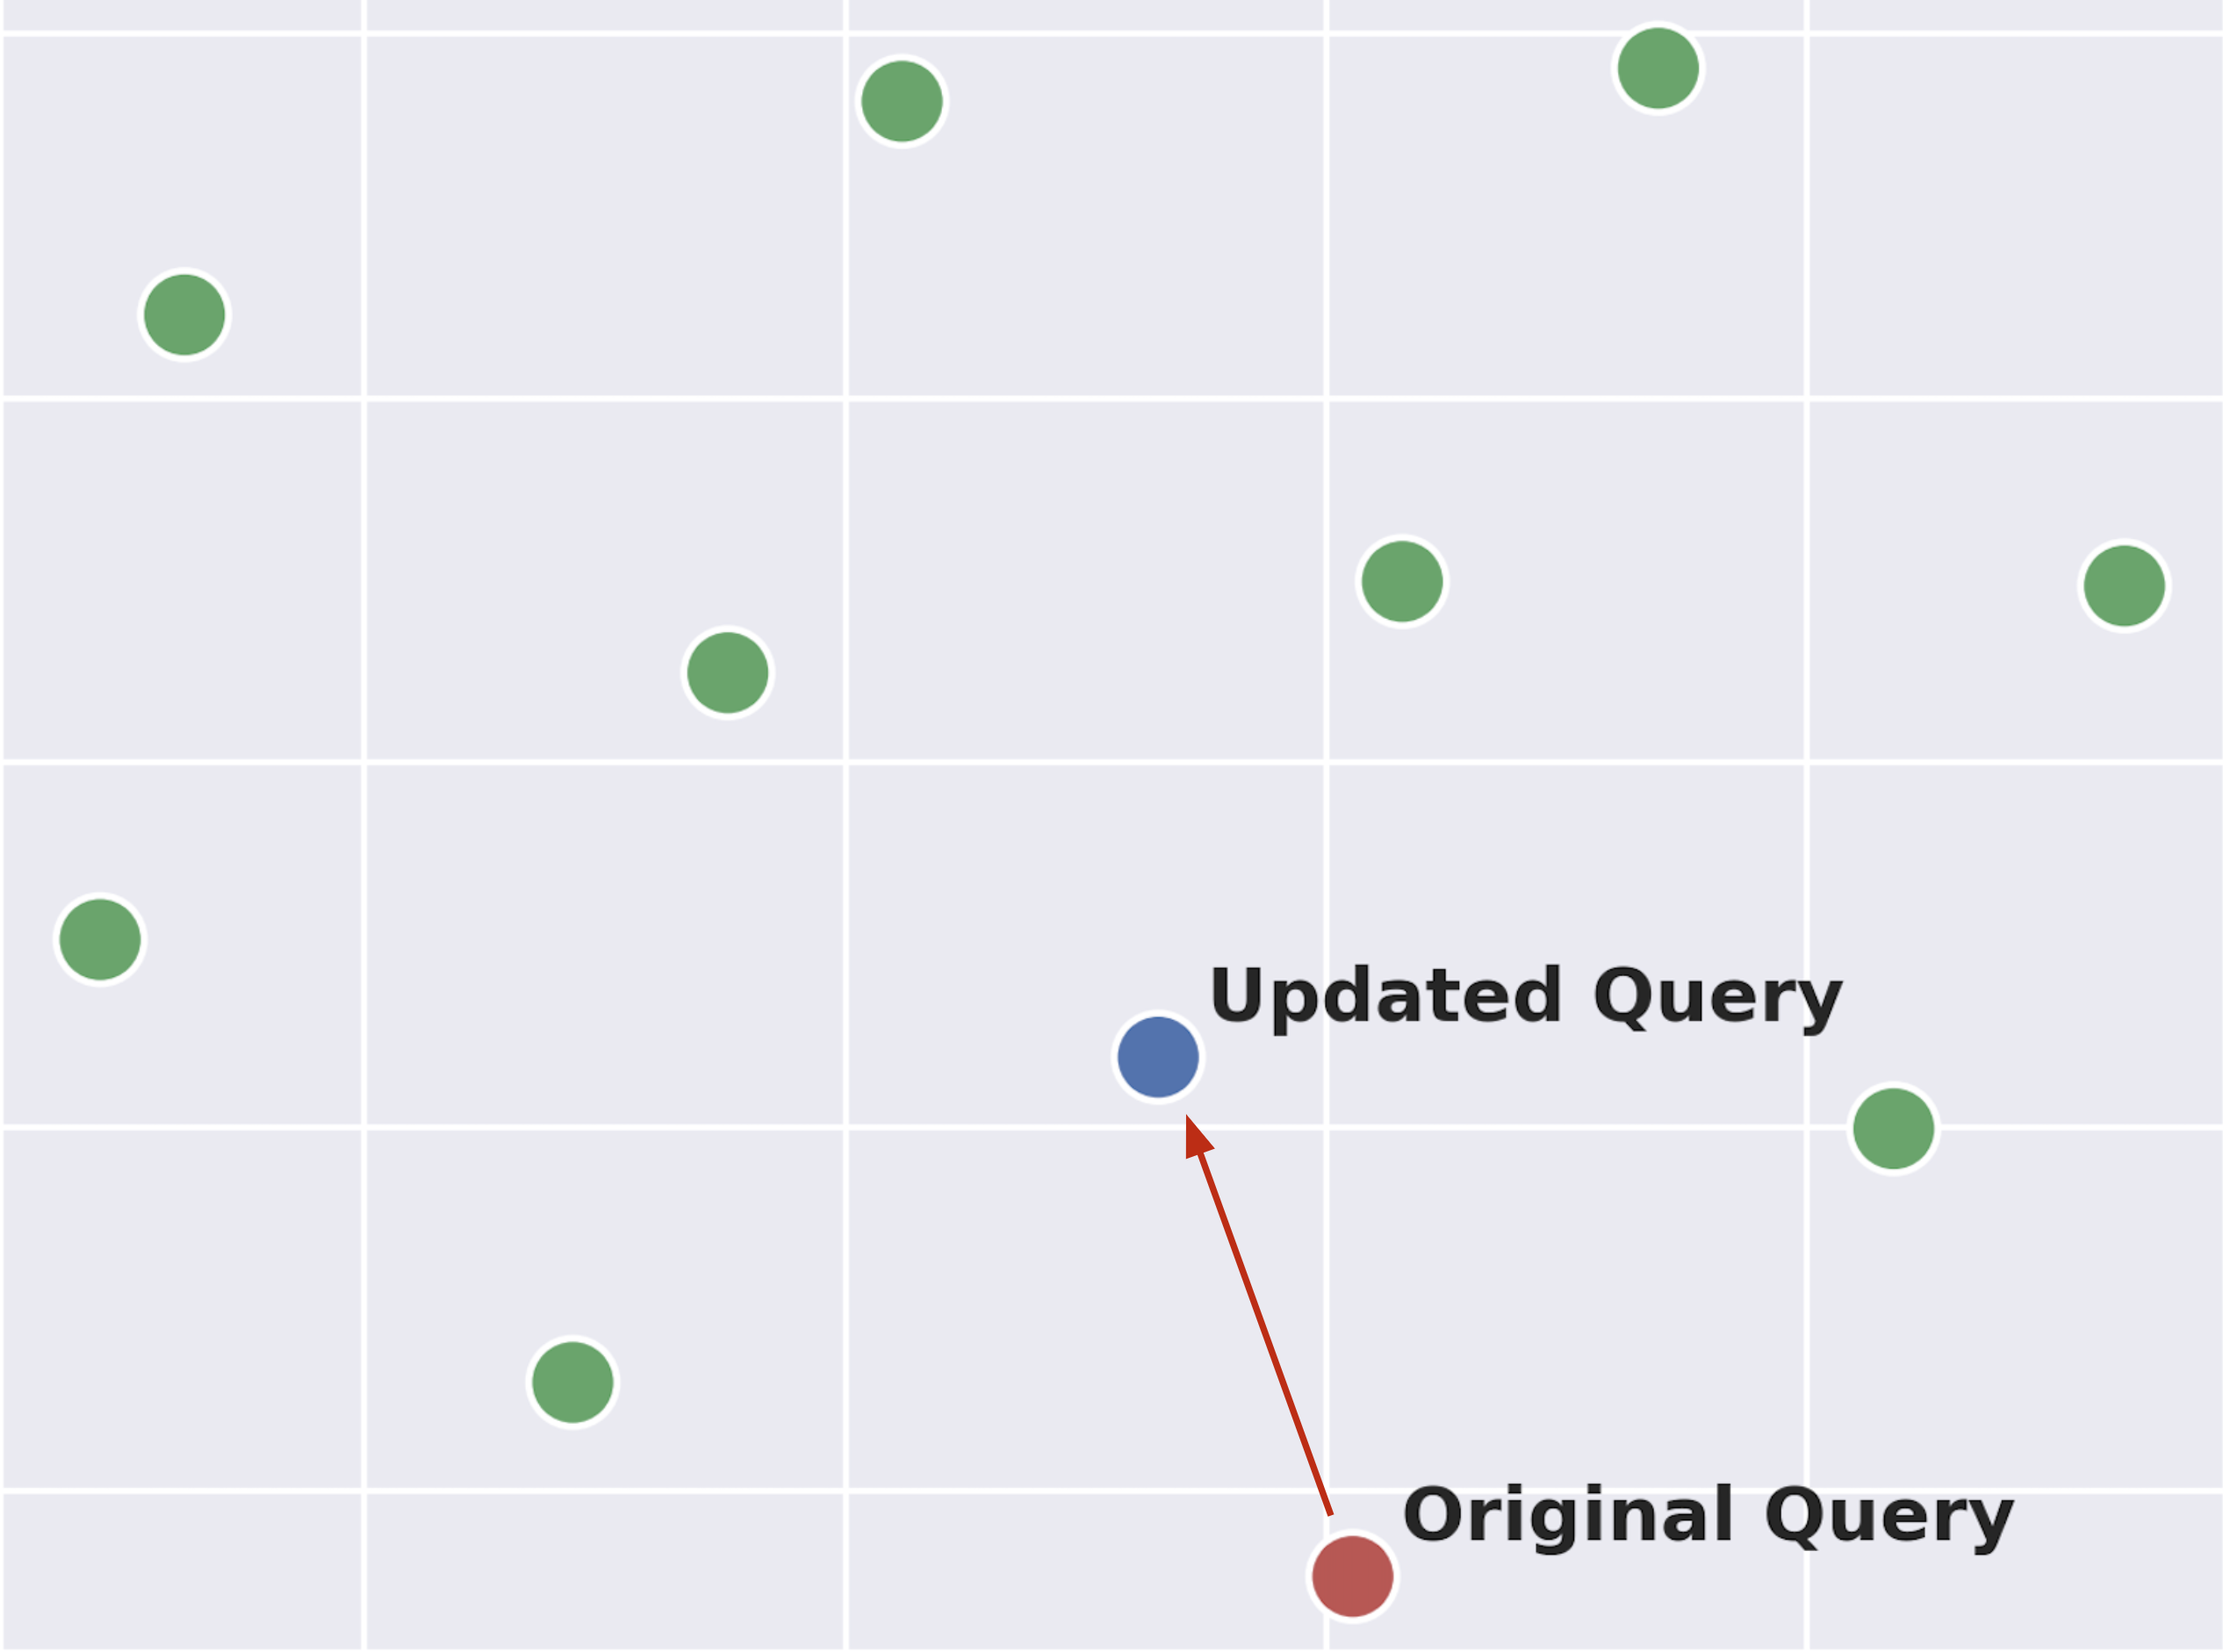
\includegraphics[width=1\linewidth]{submissions/Revanth2024/figures/qvec_1.png}
     \label{fig:qvec_1}
     %\vspace{-0.75em}
    \end{subfigure}
    \begin{subfigure}[c]{0.24\linewidth}
        \centering
     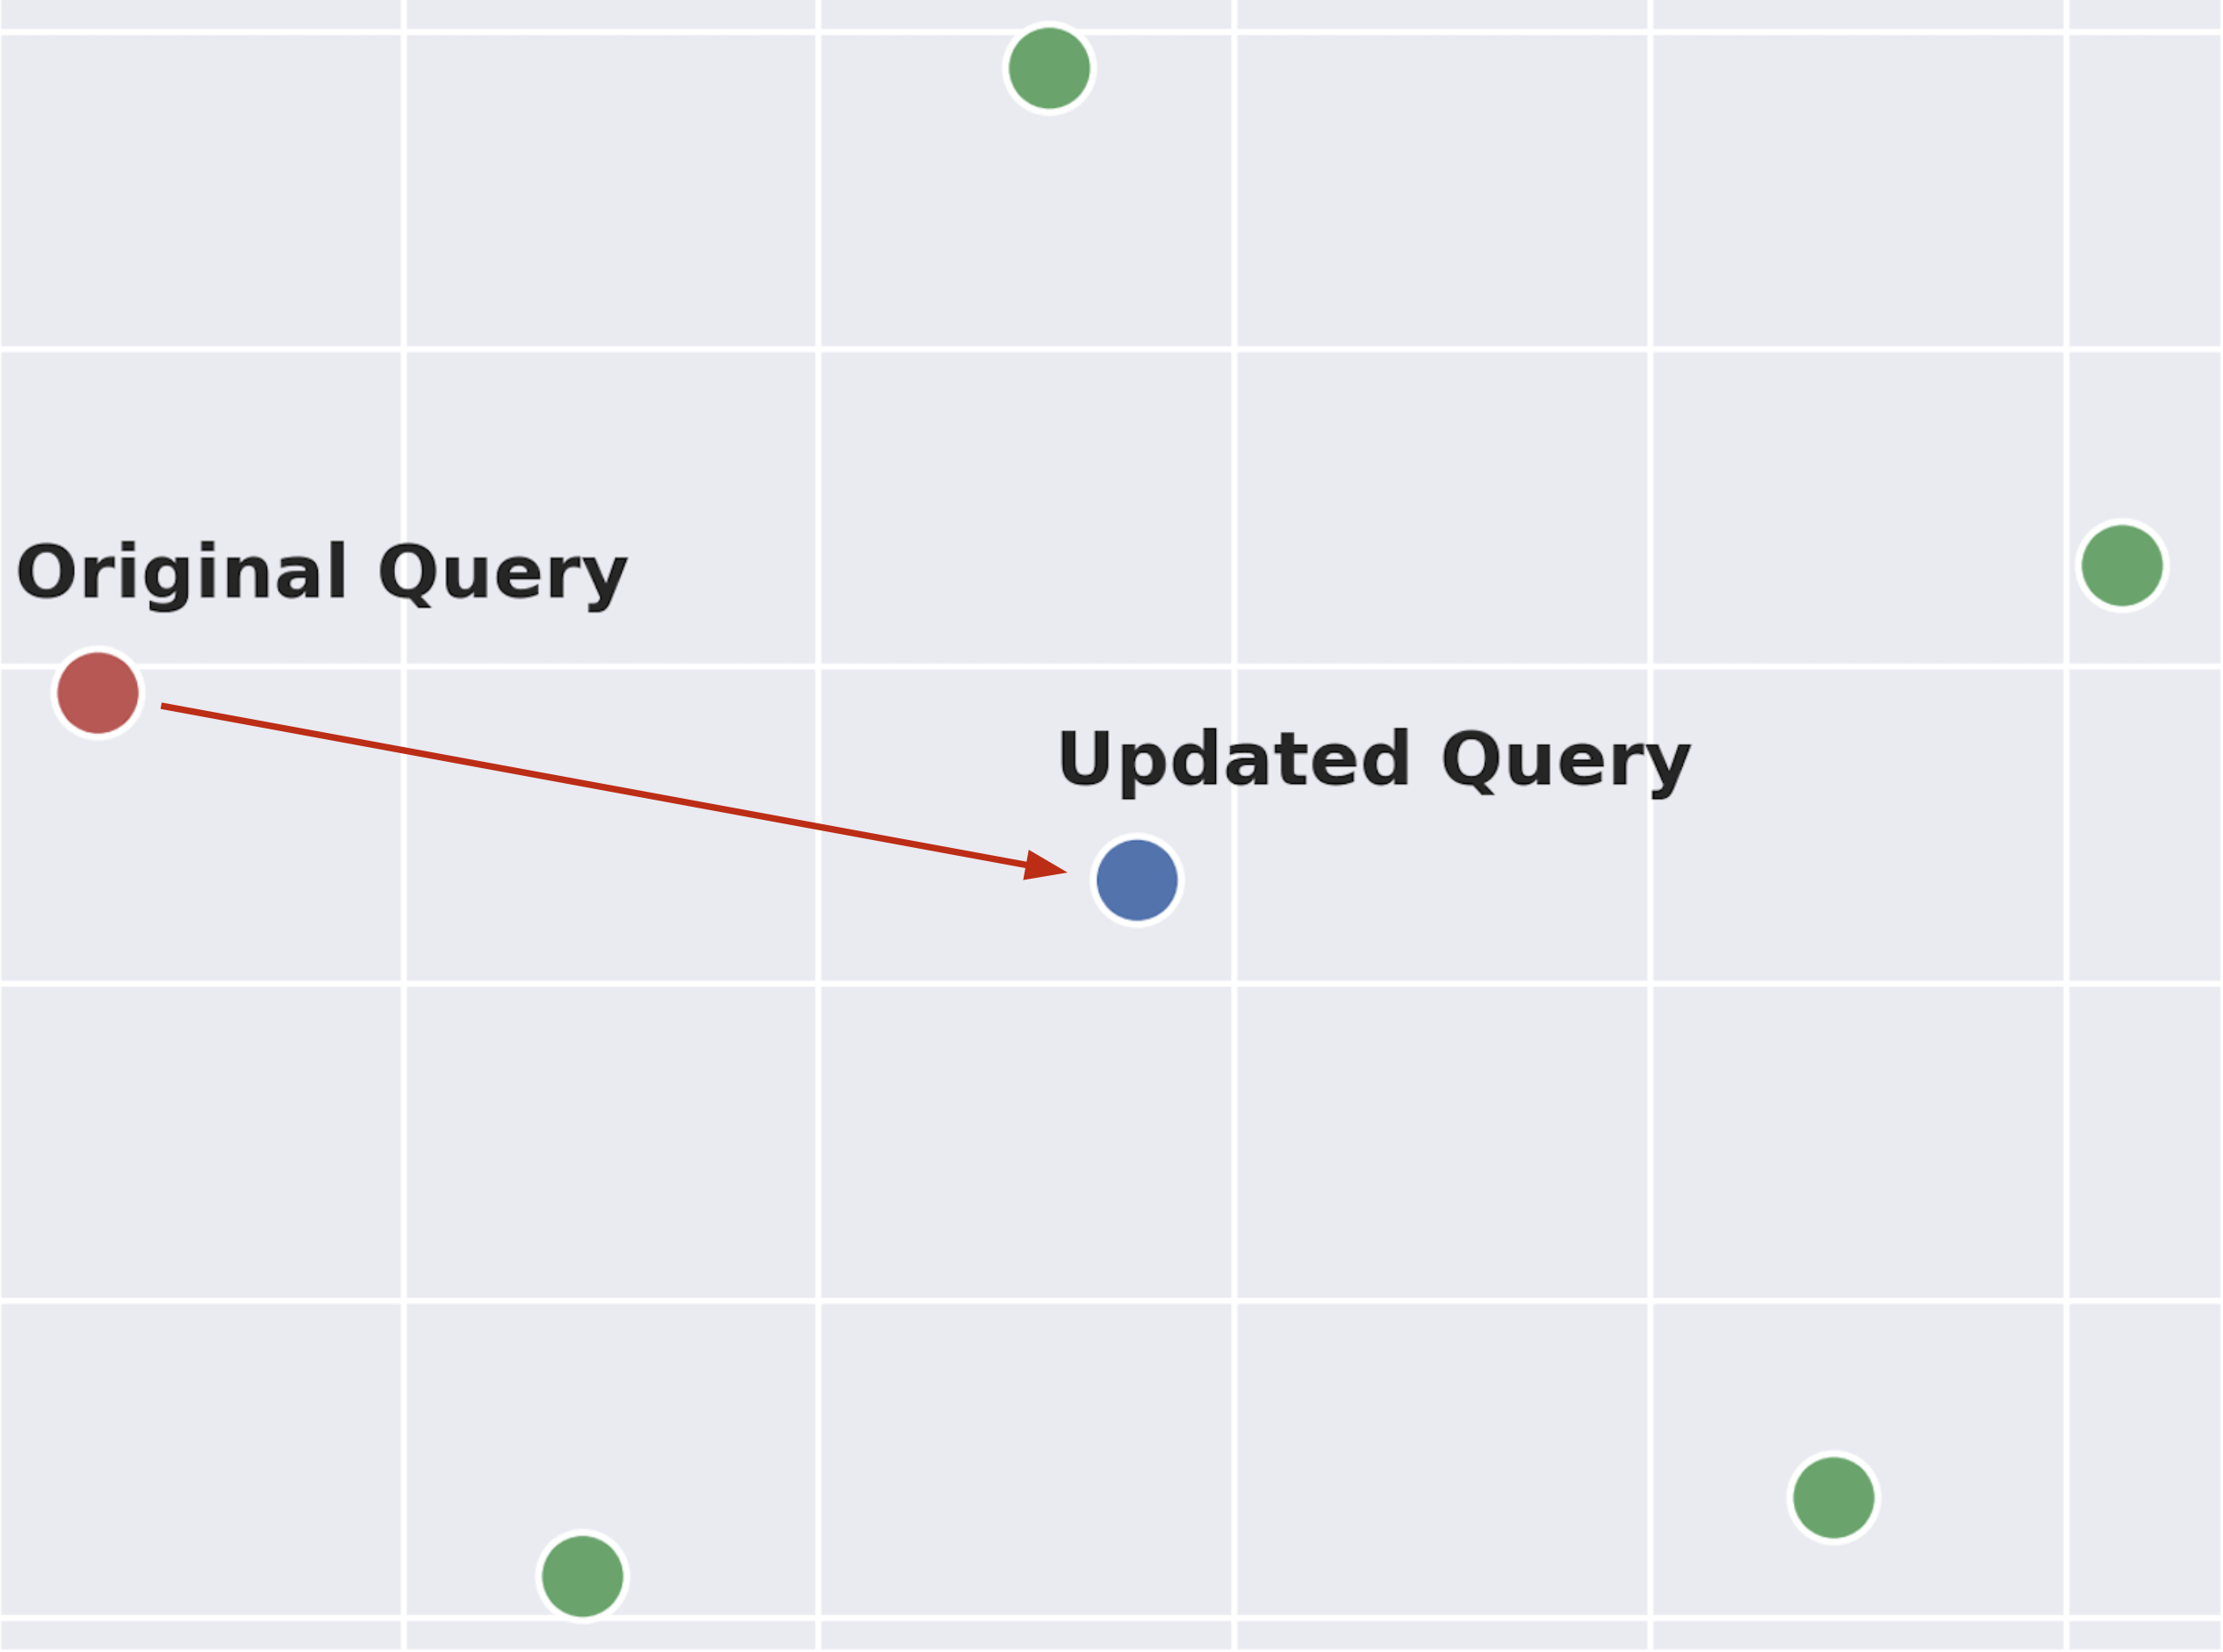
\includegraphics[width=1\linewidth]{submissions/Revanth2024/figures/qvec_2.png}
     \label{fig:qvec_1}
    %\vspace{-0.75em}
    \end{subfigure}
    \begin{subfigure}[c]{0.24\linewidth}
        \centering
     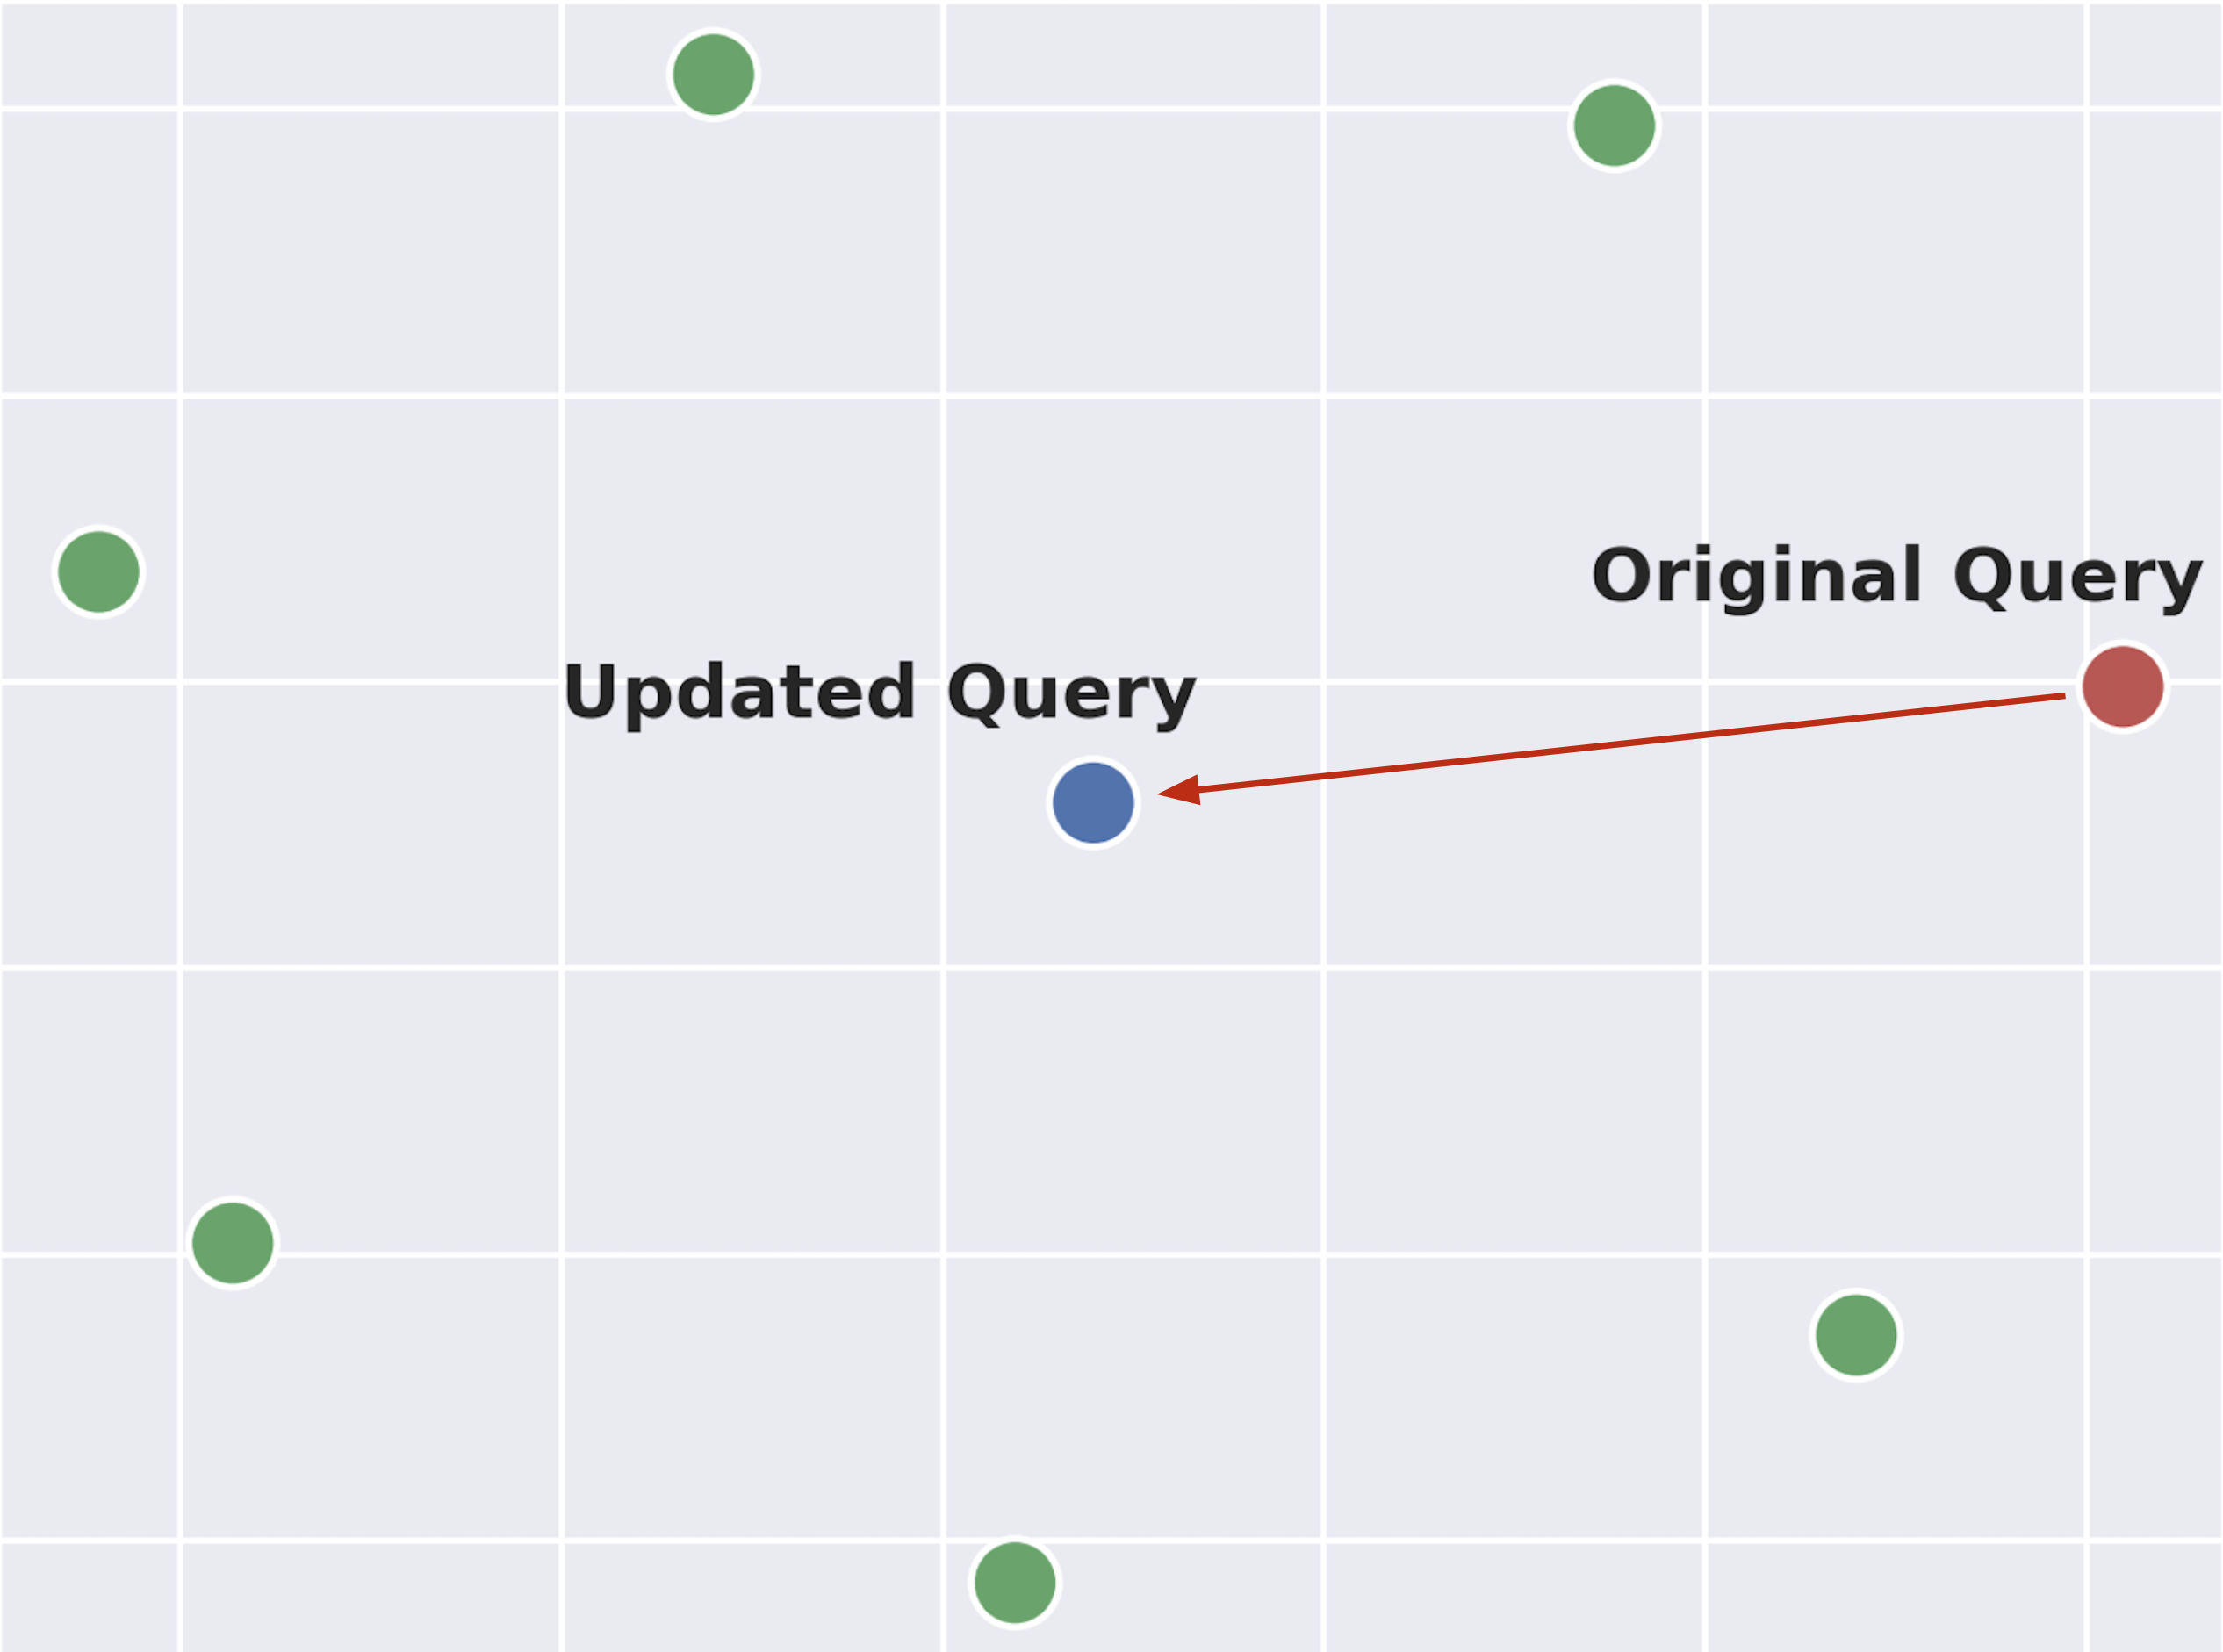
\includegraphics[width=1\linewidth]{submissions/Revanth2024/figures/qvec_3.png}
     \label{fig:qvec_1}
     %\vspace{-0.75em}
    \end{subfigure}
    \begin{subfigure}[c]{0.24\linewidth}
        \centering
     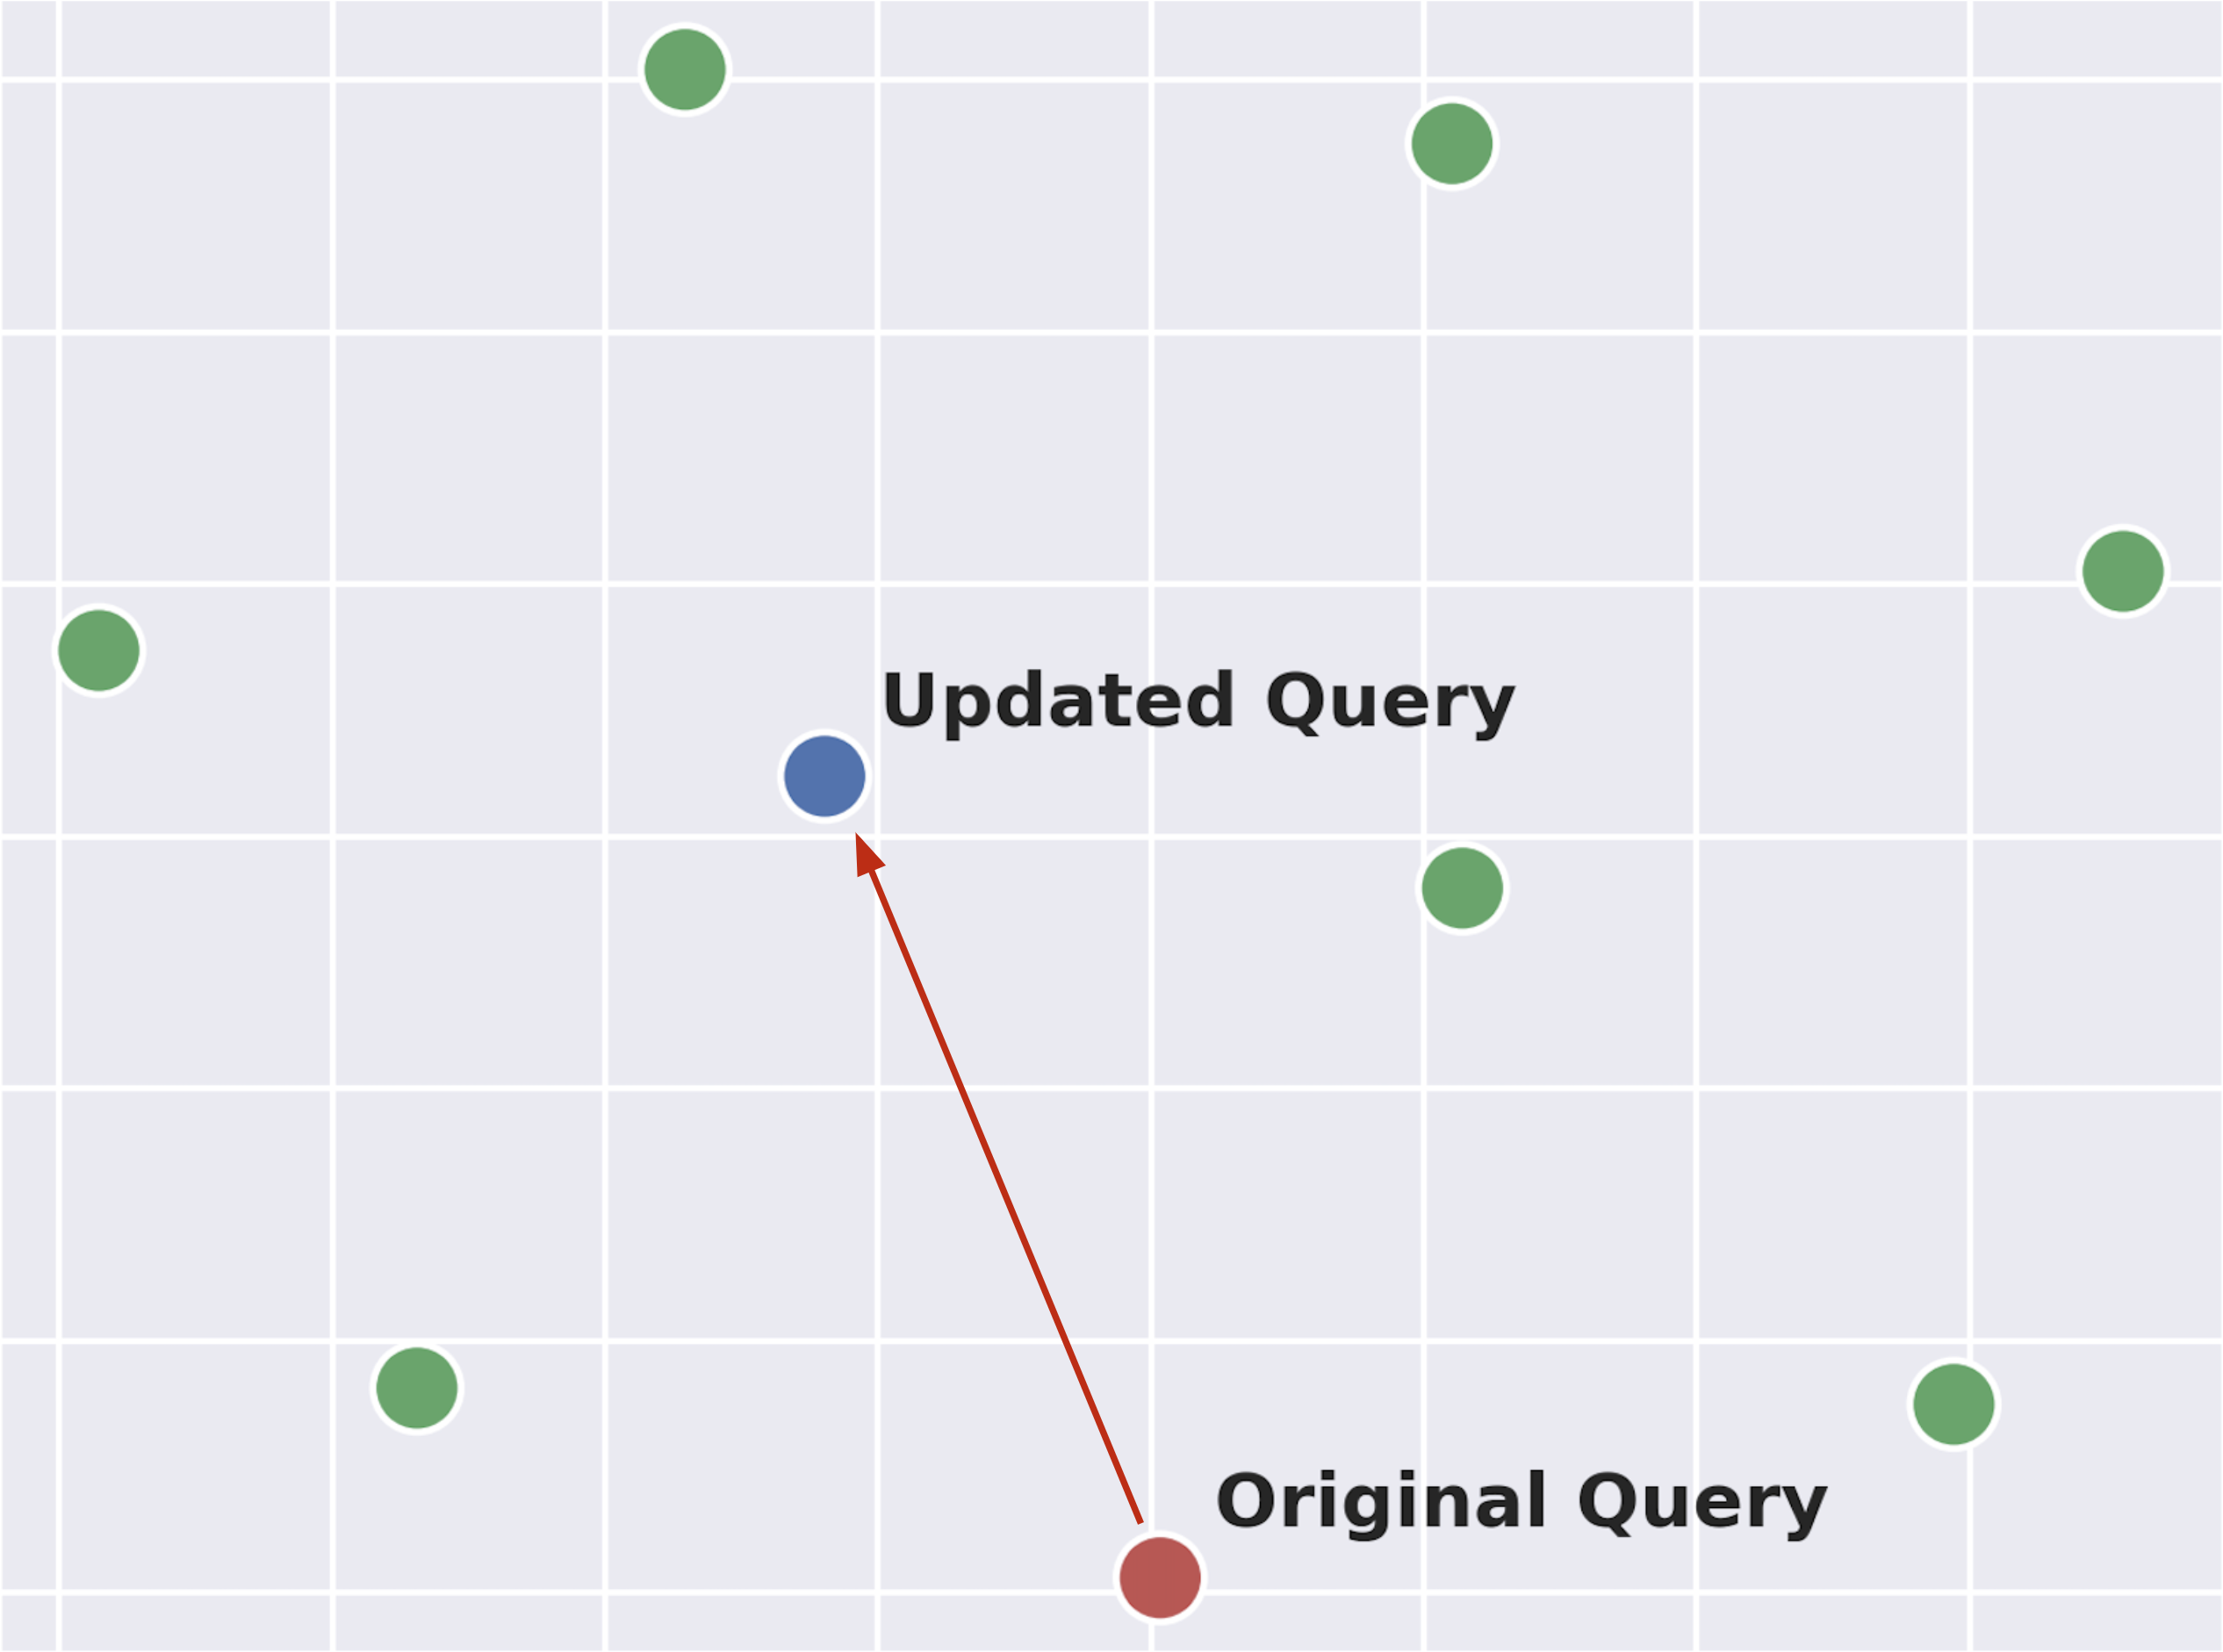
\includegraphics[width=1\linewidth]{submissions/Revanth2024/figures/qvec_4.png}
     \label{fig:qvec_1}
    %\vspace{-0.75em}
    \end{subfigure}    
    \vspace{-1.5em}
    \caption{t-SNE plots for some examples from BEIR, with the query vectors shown alongside the corresponding positive passages. The updated query vectors after \textsc{ReFIT} are now closer to the positive passages (in green).}
    \label{fig:TSNE}
\end{figure}

\begin{table}[t]
    \scriptsize
    \centering
    \def\arraystretch{1.3}
    \begin{tabular}{p{7em}|p{21em}|p{25em}}
    \multicolumn{1}{c|}{\textbf{Query}} & \multicolumn{1}{c|}{\textbf{Initial Retrieval (within Reranker Top-5)}}& \multicolumn{1}{c}{\textbf{Newly Retrieved Positive}} \\
    \hline
    treating tension headaches without medication & Most intermittent \colorbox{lime}{tension-type headaches} are easily treated with over-the-counter medications, including: 1 Aspirin. 2 Ibuprofen (Advil, Motrin IB, others) 3 Acetaminophen (Tylenol, others) & Instead of popping a pill when you get a headache, toss some almonds. For everyday \colorbox{lime}{tension-type headaches}, \textcolor{red}{almonds can be a natural remedy and a healthier alternative to other medicine}. \\
    \hline
    who drives the number 95 car in nascar & On October 2013, it was announced that McDowell would be moving to \colorbox{lime}{Leavine Family Racing's No. 95 Ford} for the 2014 \colorbox{lime}{NASCAR Sprint Cup Series} season. McDowell failed to qualify for the Daytona 500. & \textcolor{red}{Michael Christopher McDowell} is an American professional stock car racing driver. He currently competes full-time in the Monster Energy \colorbox{lime}{NASCAR Cup Series}, driving the \colorbox{lime}{No. 95 Chevrolet SS for Leavine Family Racing}. \\
    \hline
    who plays addison shepherd on grey's anatomy & In 2005, she was cast in her breakout role in the \colorbox{lime}{ABC series Grey's Anatomy, as Dr. Addison} \colorbox{lime}{Montgomery}, the estranged spouse of Derek Shepherd. & \textcolor{red}{Kathleen Erin Walsh} is an American actress and businesswoman. Her roles include \colorbox{lime}{Dr. Addison Montgomery on the ABC television} \colorbox{lime}{dramas Grey's Anatomy} and Private Practice.\\
    \hline
    \end{tabular}
    % \vspace{-1em}
    \caption{Examples of how initial retrievals highly ranked (top-5) by the reranker (middle) helps retrieve new positives (right) via the updated query vector, due to important lexical and semantic overlap (highlighted in green). The text that contains the answer to the query is shown in red.} 
    \label{tab:examples}
\end{table}


\subsection{Query vectors: the original and the new}
\label{sec:query-vectors-orig-new}

To better understand how the updated query vector after reranker relevance feedback improves recall, we take a closer look at the query and passage vectors computed for a set of BEIR examples.
Figure \ref{fig:TSNE} shows t-SNE plots for four such examples, where each dot represents a vector, and the distance between any two points is their cosine distance.
As the figure shows, the reranker feedback brings the query vector in each case closer to the corresponding positive passage vectors, making the query align with an increased number of relevant passages and consequently improving recall.
Across different datasets in BEIR, we observed that the new query vector is also closer to the initially retrieved positives by 5-16\%.

We observe that the new positives discovered by the updated query vector are closest to a passage in the reranker's top 5 in 26\% of the cases (38\% for top 10; 55\% for top 20), confirming an effective transfer of the reranker's knowledge into the query vector.
Table \ref{tab:examples} provides some examples, showing how specific words and phrases in a passage within the reranker top-5 help retrieve additional candidates with lexical/semantic overlap (highlighted in green) via relevance feedback.
Interestingly, in the fourth example, an incorrect passage highly scored by the reranker leads to the subsequent retrieval of an actual positive candidate.

\begin{figure}[t]
    \centering
    \begin{subfigure}[c]{0.32\linewidth}
        \centering
     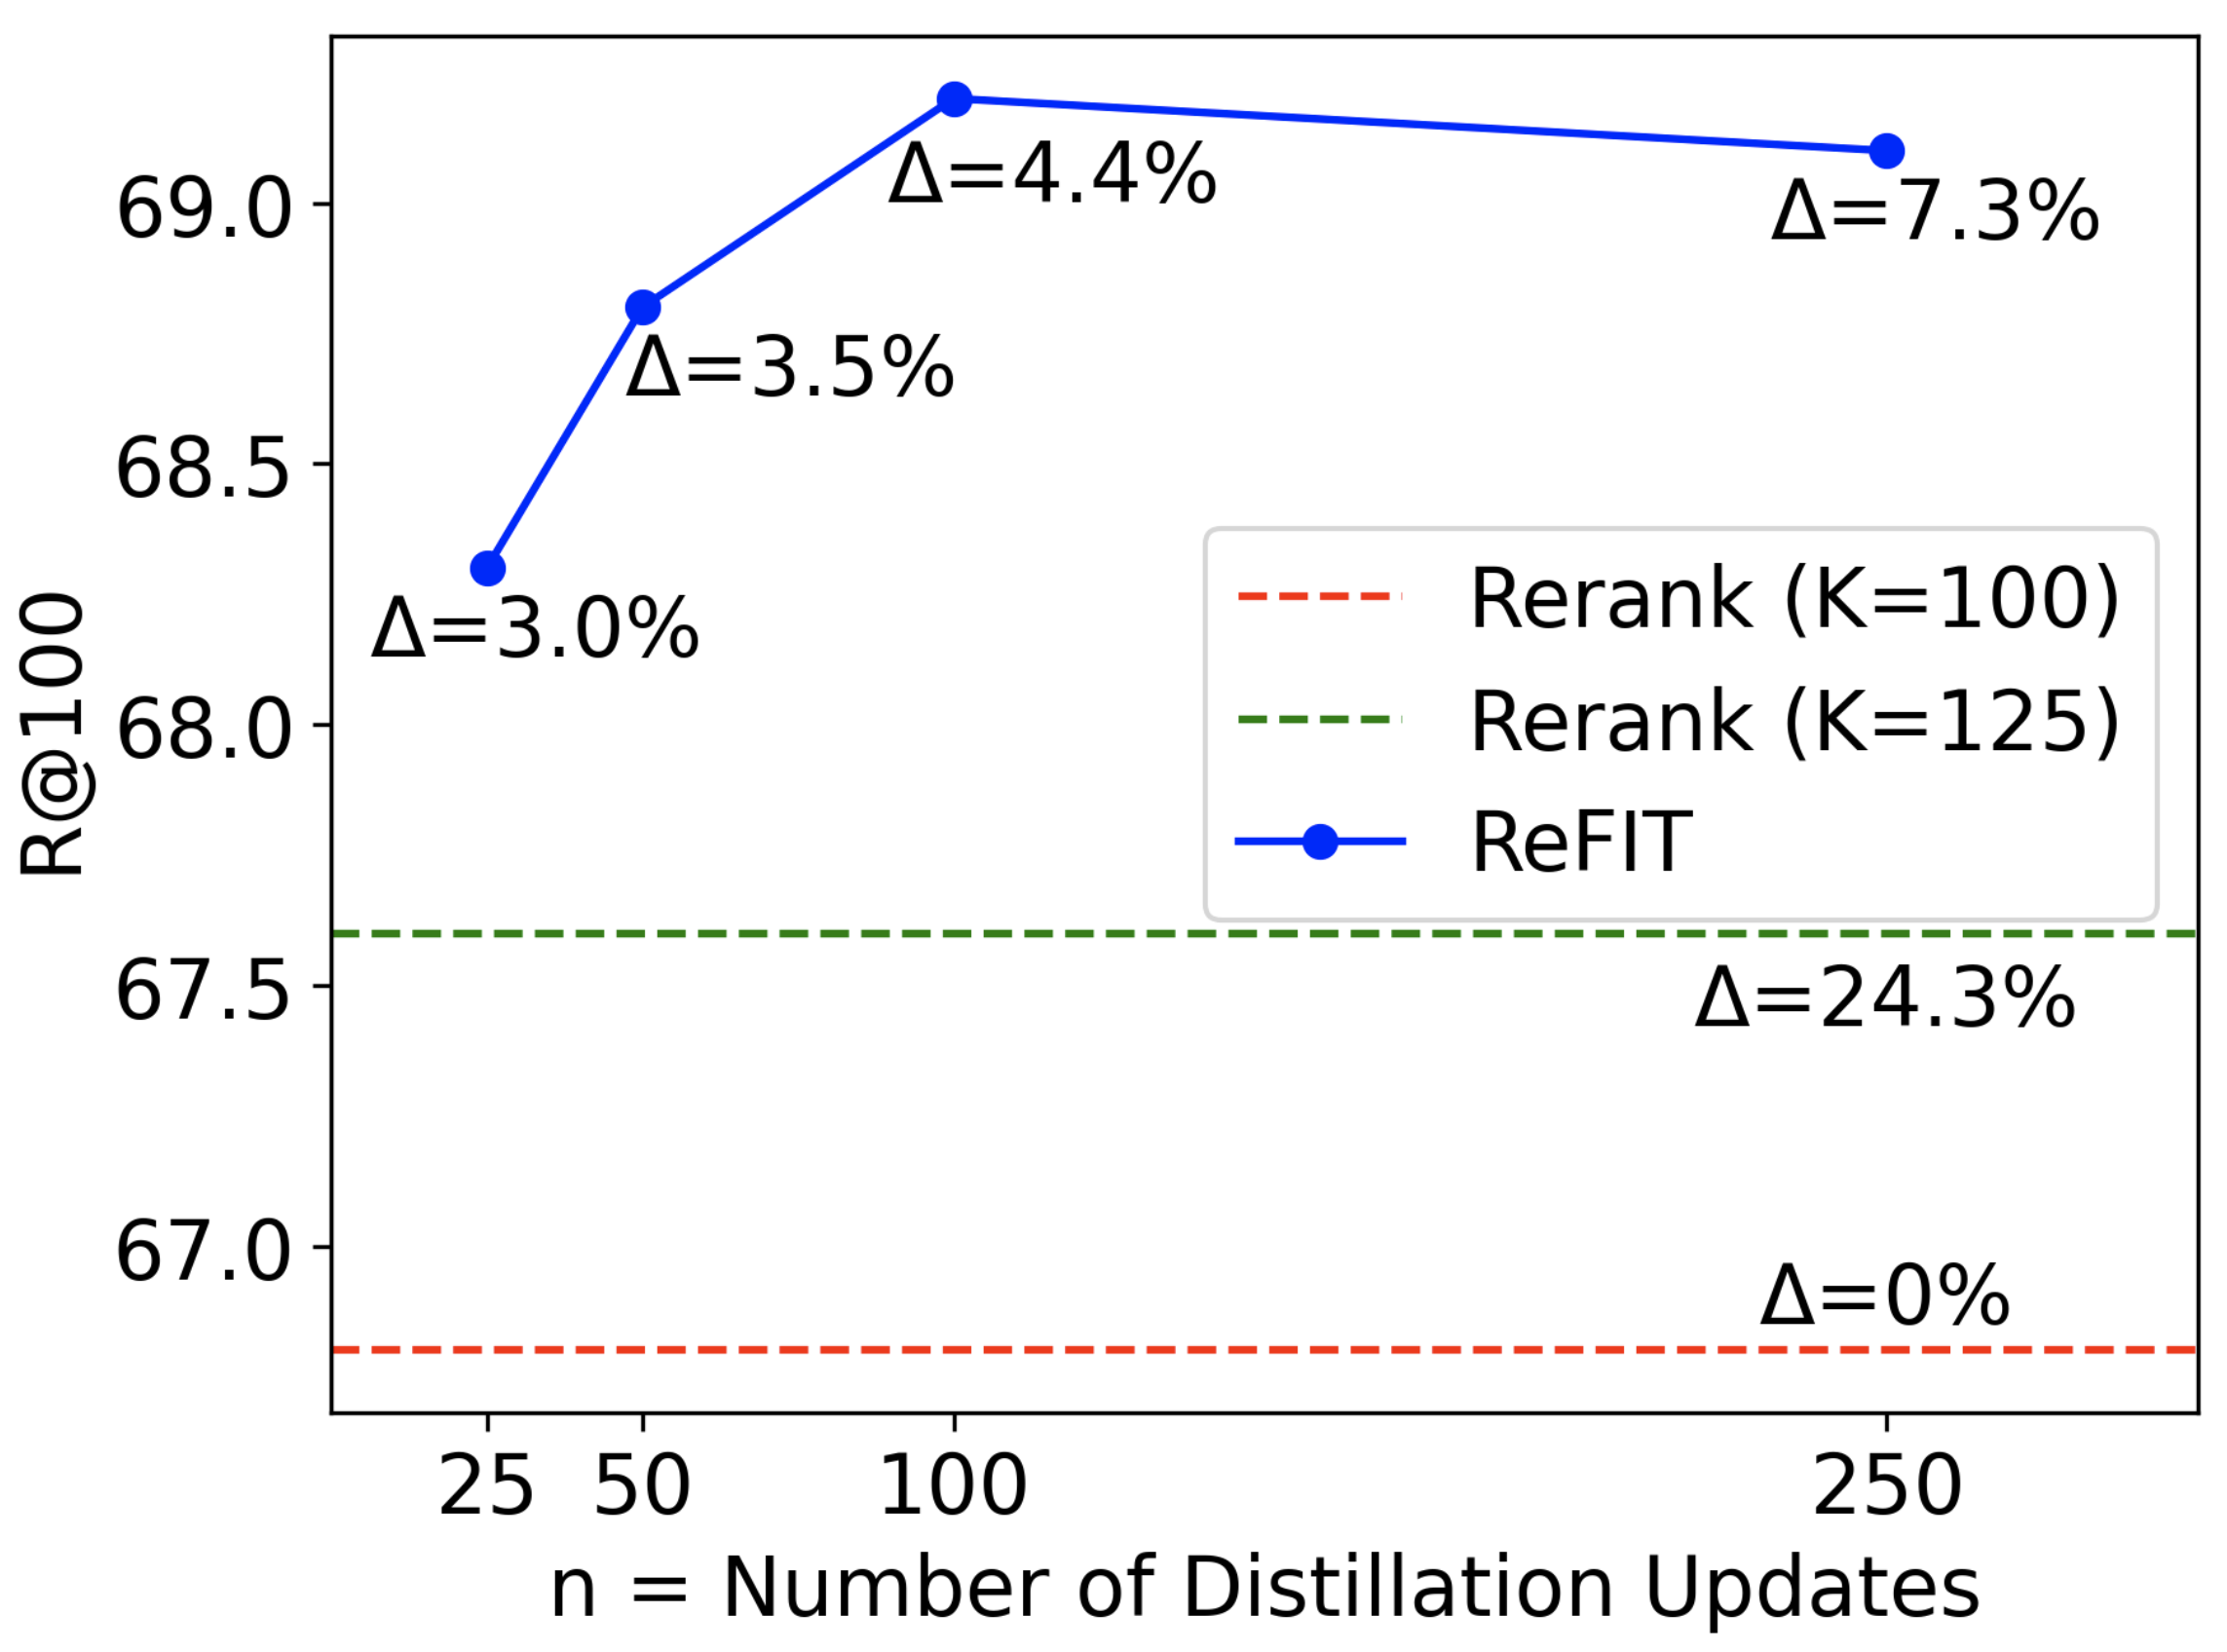
\includegraphics[width=0.95\linewidth]{submissions/Revanth2024/figures/n_variation.png}
     \label{fig:qvec_1}
     \end{subfigure}
     \hfill
     \begin{subfigure}[c]{0.32\linewidth}
        \centering
     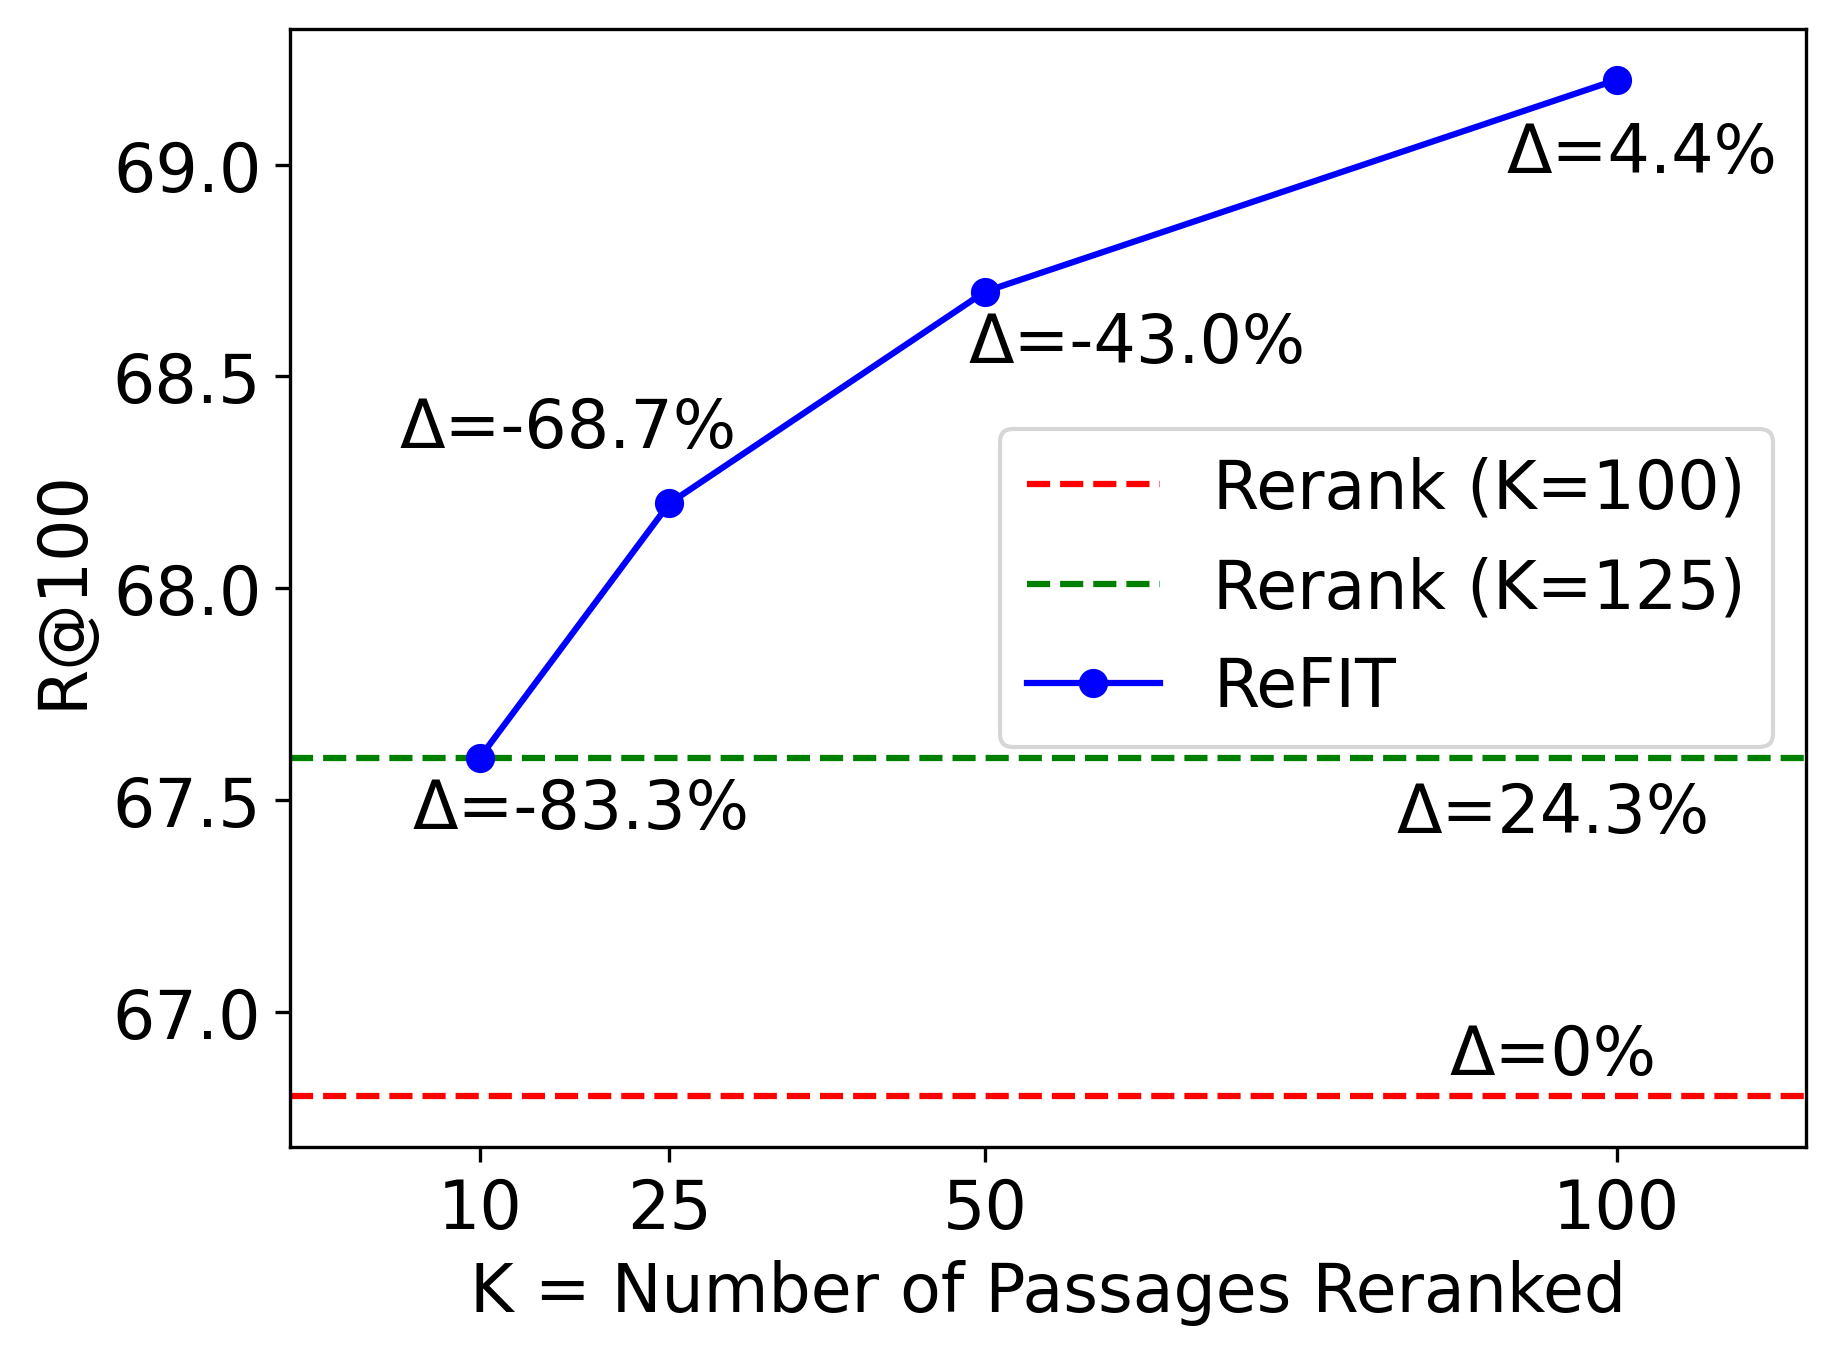
\includegraphics[width=0.95\linewidth]{submissions/Revanth2024/figures/K_variation_new.png}
     \label{fig:qvec_1}
     \end{subfigure}
     \hfill
     \begin{subfigure}[c]{0.32\linewidth}
        \centering
     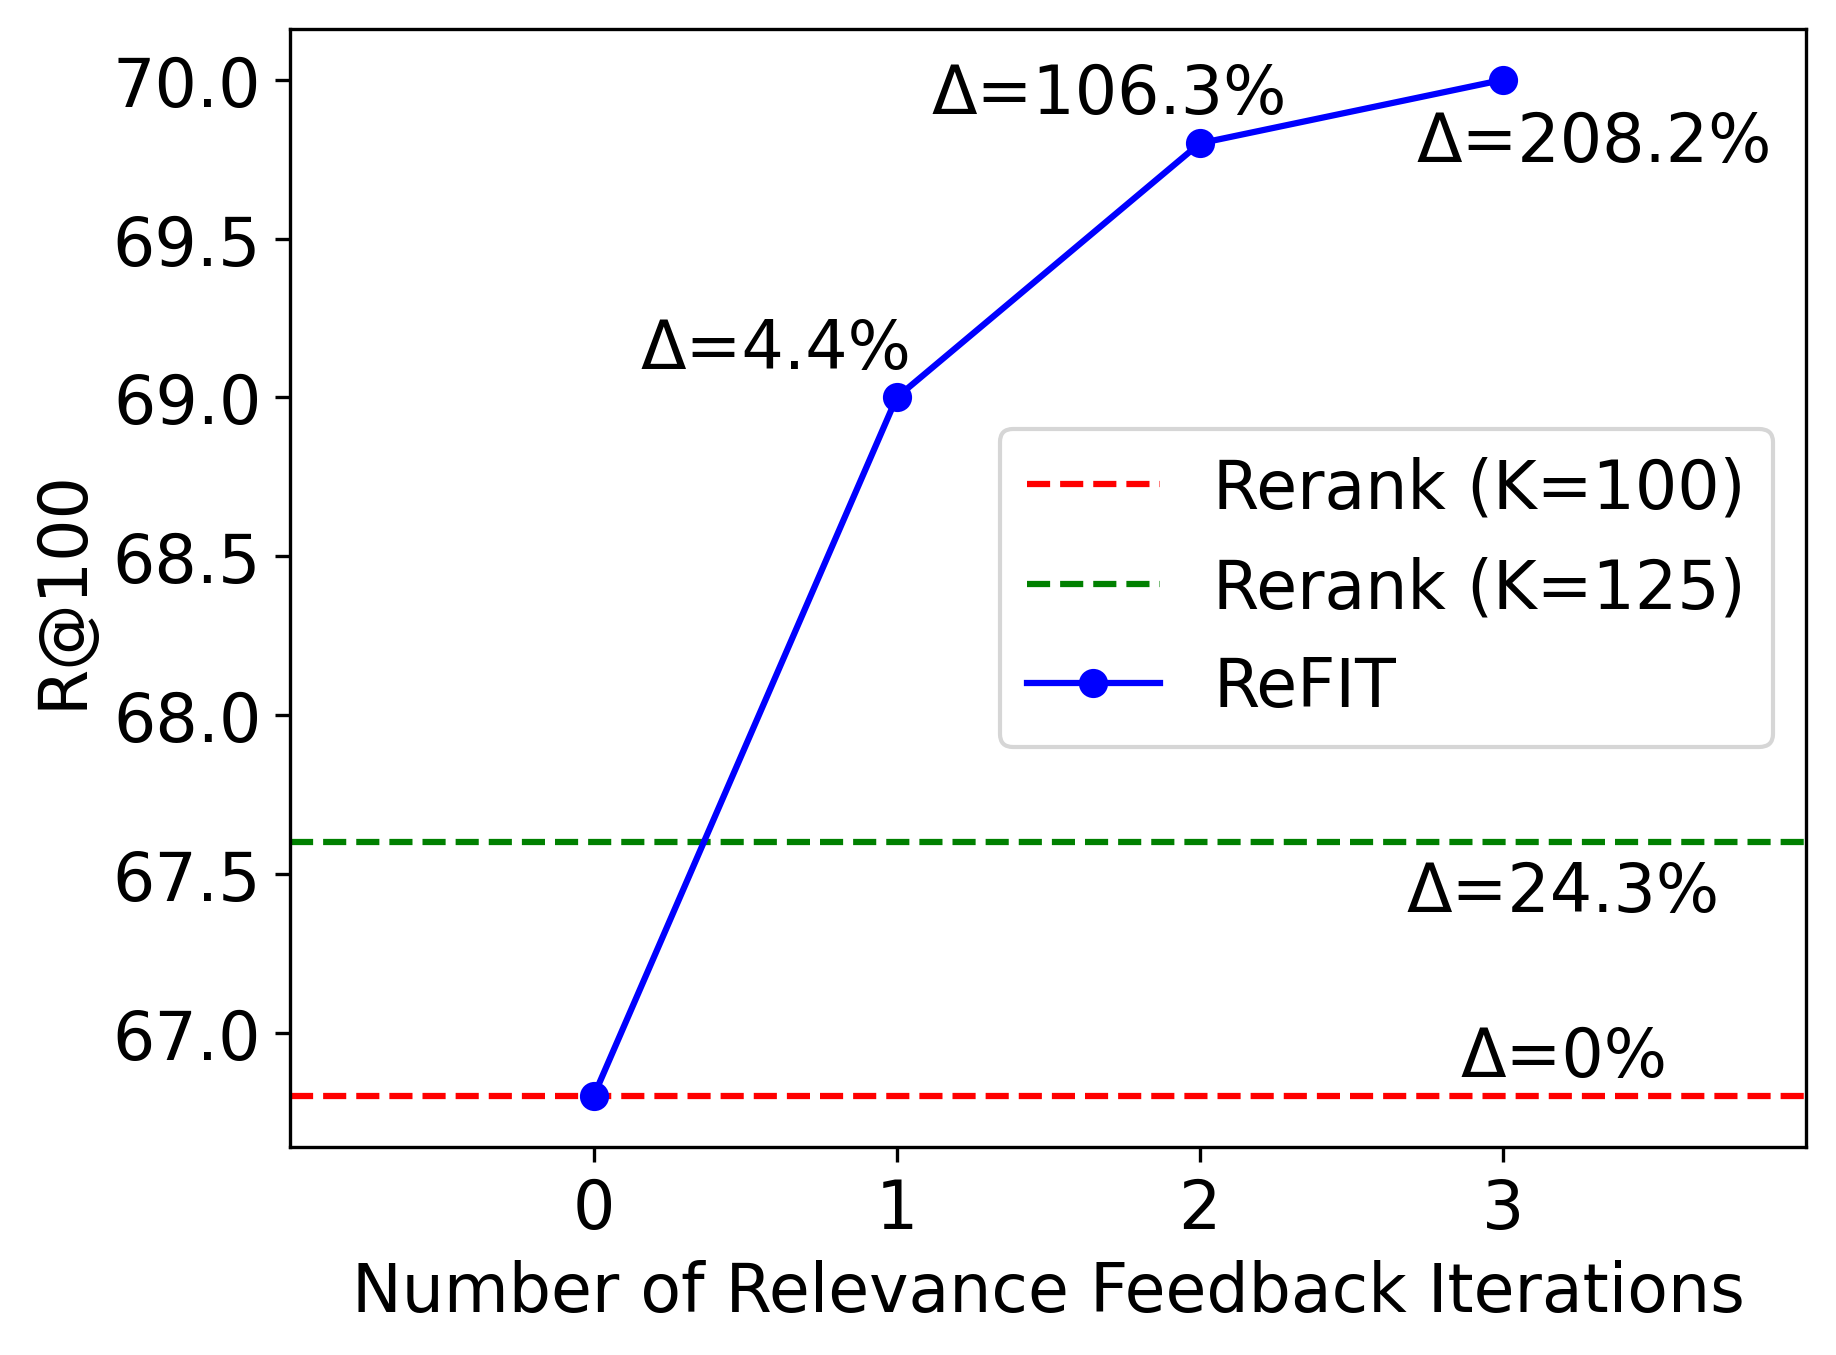
\includegraphics[width=0.95\linewidth]{submissions/Revanth2024/figures/num_iter_variation.png}
     \label{fig:qvec_1}
     \end{subfigure}
     \vspace{-0.5em}
    \caption{Variation of \textsc{ReFIT} performance with distillation updates $n$ (left), reranked passages $K$ used for distillation supervision (center) and relevance feedback iterations (right). $\Delta$ corresponds to change in latency with respect to the standard R\&R framework with $K$=100 (CPU-only configuration).}
    \label{fig:latency_performance}
    %\vspace{-0.4em}
\end{figure}


\subsection{How much additional latency does our approach introduce?}
\label{sec:additional_latency}

Our proposed method introduces a distillation and an additional retrieval step into the standard R\&R framework. While retrieval takes constant time with respect to the number of updates $n$ in Algorithm \ref{alg4}, the latency of distillation is directly proportional to $n$. Figure \ref{fig:latency_performance} (left) demonstrates the effect of varying $n$ on both the latency and performance of our approach. The extra latency is computed with respect to a standard R\&R framework that runs with $K$=100.
With a mere 4.4\% increase in latency (for when $n$=100), our method produces a gain that is significantly larger than a more computationally expensive reranking of $K$=125 candidates which in turn corresponds to 24.3\% increase in latency on a CPU. Thereby, we demonstrate that, under latency constraints, our approach can be made faster by simply lowering the number of updates, while still surpassing the conventional strategy of reranking a larger pool of candidates for improving recall.


\subsection{How do smaller $K$ values affect results?}

Our experiments described thus far are run in the standard setting of $K$=100: 100 passages are retrieved, reranked  and subsequently used to distill the reranker score distribution into the new query. Here we investigate how \textsc{ReFIT} performs as we vary $K$. Smaller values of $K$ correspond to a faster R\&R pipeline (as lower number of candidates are reranked), but it comes at the expense of the target teacher distribution now providing lesser supervision.
Figure \ref{fig:latency_performance} (center) shows Recall@100 of the post-relevance feedback retrieval step on BEIR for different values of $K$.
While a higher $K$ expectedly leads to a higher recall in general, we observe performance improvements over directly reranking 125 passages, even when considerably smaller number of passages are used for distillation.
Our approach can thus be easily tuned to achieve different accuracy-speed trade-offs depending on the requirements of the target application.


\subsection{Can multiple iterations of relevance feedback further improve results?}
\label{sec:multi_iterations}
Our relevance feedback approach improves recall when the updated query vector is used for a second retrieval step. 
Here we examine if further improvements are possible from more iterations of relevance feedback, i.e., running the following operations in a loop: (1) rerank the retrieval results from the previous iteration, (2) update the query vector via distillation from the reranker distribution, and (3) retrieve again. We note that this experiment operates under the assumption of a relaxed time budget, as the computationally expensive reranker must be executed $N$ times.
Figure \ref{fig:latency_performance} (right) shows performance on BEIR from $N$ iterations of relevance feedback, with $N=0$ corresponding to baseline retrieval. We can see that recall improves with each additional round of relevance feedback; the biggest gain comes in the first round ($N=1$) and performance saturates after $N=2$.

\subsection{Further Discussion}
\subsubsection{The curious case of zero initial positives:} In \S{\ref{sec:query-vectors-orig-new}}, we presented an example where our method leverages a close negative among the initially retrieved candidates to later retrieve a positive passage. We find that in 24\% of the cases where the first-stage retriever retrieves no positive passages, our method can improve recall in a similar fashion. Among all cases where recall improves, however, 75\% have at least one positive in the top retrieved results. These results indicate that while the presence of positive candidates in the initial retrieval is useful, our relevance feedback approach can also generally leverage informative negatives to update the query vector in the right direction.

\subsubsection{Choice of Reranker:}
In the experiments comparing our approach to the R\&R framework, we used an efficient (yet high-performing) reranker both in the baseline model and as the teacher model for distillation. Would the results have been different if we used a more powerful (but computationally expensive) reranker instead?
To find an answer, it is essential to note that the final recall of an R\&R engine is inherently limited by the underlying retriever. For instance, the Recall@100 of an R\&R pipeline with $K$$=$$125$ cannot exceed the Recall@125 of the underlying retriever, irrespective of the quality of the reranker. The Recall@100 of \textsc{ReFIT} (BEIR: 69.2, Mr. TyDi: 89.7, MKQA: 68.2 and MSRVTT: 92.9) is consistently higher than the Recall@125 of the baseline retriever (BEIR: 68.9,  Mr. TyDi: 88.2, MKQA: 66.9 and MSRVTT: 92.8). These results clearly suggest that even the best reranker baseline would fail to attain the recall of our method. Further, we can expect a better reranker to improve the recall of \textsc{ReFIT} since leveraging a stronger teacher model for distillation should lead to a better student (retriever query vector).